% LaTeX rebuttal letter example. 
% 
% Copyright 2019 Friedemann Zenke, fzenke.net
%
% Based on examples by Dirk Eddelbuettel, Fran and others from 
% https://tex.stackexchange.com/questions/2317/latex-style-or-macro-for-detailed-response-to-referee-report
% 
% Licensed under cc by-sa 3.0 with attribution required.

\documentclass[11pt]{article}
\usepackage{amsmath}
\usepackage[sorting = none]{biblatex}
\usepackage{xcolor}
\usepackage{color}
\usepackage{tcolorbox} % Frames
\usepackage{booktabs} % For \toprule, \midrule, etc.
\tcbuselibrary{theorems}
\tcbuselibrary{breakable}
\usepackage{enumitem}
\usepackage{caption}
\usepackage{tikz}
\usetikzlibrary{positioning, arrows.meta, decorations.pathreplacing, calc}
\usepackage{cleveref} % references in tcolorboxes
\usepackage{amsthm}
\newtheorem*{remark}{Remark}
\newtheorem{theorem}{Theorem}
\usepackage{enumitem}
\usepackage{calc} % for \widthof


\addbibresource{First_Article_References_Short_List.bib}
\usepackage{amsmath}
\usepackage{amsfonts}
\usepackage[utf8]{inputenc}
\usepackage{algorithmic}
\usepackage[noend]{algorithm2e}
\usepackage[framemethod=TikZ]{mdframed}
\usepackage{booktabs}
\usepackage{xcolor}
\global\mdfdefinestyle{Resp}{%
    linecolor=gray,
    outerlinewidth=0pt,
    roundcorner=5pt,
    innertopmargin=5pt,
    innerbottommargin=5pt,
    innerrightmargin=10pt,
    innerleftmargin=10pt,
    backgroundcolor=gray!10!white,
    }

\usepackage{fullpage}
%\newcommand\arash[1]{\textcolor{red}{#1}}

\usepackage{multirow}
% import Eq and Section references from the main manuscript where needed
% \usepackage{xr}
% \externaldocument{manuscript}
\usepackage{lineno}
% package needed for optional arguments
\usepackage{xifthen}
% define counters for reviewers and their points
\newcounter{reviewer}
\setcounter{reviewer}{0}
\newcounter{point}[reviewer]
\setcounter{point}{0}


% This refines the format of how the reviewer/point reference will appear.
\renewcommand{\thepoint}{\thereviewer.\arabic{point}} 

% command declarations for reviewer points and our responses
\newcommand{\reviewersection}{\stepcounter{reviewer} \bigskip \hrule
                  \section*{Reviewer \thereviewer}}

\newenvironment{point}
   {\refstepcounter{point} \bigskip \noindent {\textbf{Reviewer Point~\thepoint} } ---\ }
   {\par }

\newcommand{\shortpoint}[1]{\refstepcounter{point}  \bigskip \noindent 
	{\textbf{Reviewer~Point~\thepoint} } ---~#1\par }
	


% \newenvironment{reply}
%    {\medskip \noindent
%    \begin{sf}\textbf{Reply}:\  }
%    {\medskip \end{sf}}
% Reply counter resets for each reviewer
\newcounter{replyctr}[reviewer]

\renewcommand{\thereplyctr}{\thereviewer.\arabic{replyctr}}

\newenvironment{reply}
  {\refstepcounter{replyctr}% STEP FIRST
   \addtocounter{replyctr}{-1}% MOVE BACK TO PRINT .0
   \medskip\noindent
   \begin{sf}\textbf{Reply~\thereplyctr:}\ }
  {\addtocounter{replyctr}{1}% MOVE FORWARD FOR NEXT REPLY
   \medskip\end{sf}}



\DeclareMathOperator*{\argmax}{arg\,max}

\begin{document}

\begin{center}
\Large
\textbf{Energy-Efficient and Near Real-Time Routing Algorithm for Disaster Monitoring in Wireless Sensor Networks}\\
\vspace{0.5cm}
\large
%Ranwa Al Mallah, David Lopez, Godwin Badu-Marfo, Bilal Farooq\\
\vspace{0.25cm}
Response to the reviewers\\
\today
\end{center}
\vspace{2cm}
%\section*{Response to the reviewers}
% General intro text goes here
We would like to thank the editors and the reviewers for their careful review, constructive recommendations and positive and encouraging comments. We appreciate the time and effort that the reviewers dedicated to provide valuable feedback on our manuscript. In the following, we have listed the reviewers' comments, followed by our point-to-point responses in the gray box. In this document, texts in “bold” and blue refer to manuscript texts of the revised version of our paper
that are directly quoted here.\\ 

The summary of main changes that we have undertaken includes:
\begin{description}[leftmargin=!, labelwidth=\widthof{\textbf{Discussion and Limitations}}]
  \item[\textbf{Methodology}] The core algorithm has been substantially revised, replacing the original TSMixer with a new model that better aligns with the study’s objectives and reviewer's comments.

  \item[\textbf{Experiments}] The experimental setup has been updated accordingly, with detailed descriptions and expanded evaluations reflecting the revised methodology.

  \item[\textbf{Discussion and Limitations}] A dedicated discussion section has been added, explicitly addressing the limitations and broader implications of the proposed approach.

  \item[\textbf{Abstract}] The abstract has been significantly revised to reflect the new algorithm and updated contributions.

  \item[\textbf{Conclusion}] The conclusion has been rewritten to emphasize the broader impact of the work and outline future research directions.
\end{description}





\pagebreak
\begin{refsection}
\reviewersection
This paper proposes a hybrid multi-agent deep reinforcement learning (MADRL) approach for routing in disaster-monitoring wireless sensor networks (WSNs). The authors combine QMIX and QTRAN with a TSMixer-based forecasting mechanism to dynamically select the better-performing model at each episode, while also introducing an attention-based reward structure to better capture complex tradeoffs between energy efficiency, latency, and packet delivery ratio. A custom Gym environment with node mobility was designed for evaluation. Results show that the proposed hybrid model achieves a better balance between energy consumption, latency, and delivery reliability compared to QMIX and QTRAN individually, making it promising for near real-time disaster monitoring applications.

The paper has useful contributions, including: (i) addressing both energy efficiency and real-time performance in WSN disaster settings, (ii) combining two advanced MADRL algorithms in a novel switching framework, (iii) designing a richer attention-based reward function, and (iv) performing a comprehensive evaluation under multiple scenarios. These aspects make the work relevant and technically interesting.

However, the paper also has notable limitations.\\

\begin{mdframed}[style=Resp]
\begin{reply}\label{1:0}
We thank the reviewer for the encouraging comments. We addressed the major concerns as follows.
\end{reply}
\end{mdframed}
\textbf{Notable limitations:}

\begin{point}

First, the training parameters of the RL models (e.g., learning rate, discount factor, exploration policy) are not reported, which makes it unclear whether QMIX, QTRAN, and the hybrid were fairly trained and tuned.

\end{point}

\begin{mdframed}[style=Resp]
\begin{reply}\label{1:1}
To address the reviewer’s concern, we now provide a complete summary of the training hyperparameters (\textbf{\textcolor{blue}{Section IV, Table IV of the revised manuscript}}) used for QMIX, QTRAN, and GAPF (the hybrid model) which stands for Graph-Attentive Policy Fusion. These details ensure that the experimental setup is transparent and reproducible.
Before presenting the training hyperparameters, we first outline the methodology and architectural design of GAPF (\textbf{\textcolor{blue}{Section III.E of the revised manuscript}}), as this component is central to understanding our hybrid framework.
\subsection{GAPF: Graph-Attentive Policy Fusion}
\label{sec:gapf}

We introduce \textbf{GAPF} (Graph-Attentive Policy Fusion), a lightweight meta-algorithm that learns to select, at the episode level, the best-performing MARL expert for a given WSN topology. GAPF leverages a \emph{graph neural network} (GNN) to encode the spatial structure of the sensor network and a \emph{meta-controller} trained via REINFORCE~\cite{williams1992simple} to make a topology-informed selection between two pre-trained experts (QMIX and QTRAN).

\subsubsection{Problem Formulation}
\label{sec:gapf_formulation}

Let $\mathcal{E} = \{\pi_{\text{QMIX}}, \pi_{\text{QTRAN}}\}$ denote a set of pre-trained, frozen MARL policies, each mapping joint observations to joint actions in the WSN routing Dec-POMDP. At the start of each episode~$k$, the WSN is characterised by a communication graph $\mathcal{G}_k = (\mathcal{V}, \mathcal{E}_k)$, where nodes $\mathcal{V} = \{1, \dots, N\}$ are sensors and an edge $(i,j) \in \mathcal{E}_k$ exists if and only if $\|p_i - p_j\|_2 \leq R$, with $p_i \in \mathbb{R}^2$ the position of sensor~$i$ and $R$ the communication radius. GAPF learns a parameterised policy $\mu_\theta$ that maps the topology $\mathcal{G}_k$ to a selection decision $a^{\text{meta}}_k \in \{\text{QMIX}, \text{QTRAN}\}$, maximising the expected episodic return:
\begin{equation}
    \max_\theta \; \mathbb{E}_{\mathcal{G}_k}\!\left[\, G_k \,\middle|\, \pi_{a^{\text{meta}}_k}\right], \quad a^{\text{meta}}_k \sim \mu_\theta(\cdot \mid \mathcal{G}_k).
    \label{eq:gapf_objective}
\end{equation}

\subsubsection{Architecture}
\label{sec:gapf_architecture}

The GAPF model $\mu_\theta$ consists of two modules: (i)~a \emph{GCN encoder} that produces a fixed-dimensional graph embedding from the variable-size WSN topology, and (ii)~a \emph{CAS controller} (Contextual Algorithm Selection) that maps this embedding to a Bernoulli selection probability. The full architecture is illustrated in Figure~\ref{fig:gapf_architecture} and detailed below.

\paragraph{Graph construction.}
Given the $N$ sensor positions $\{p_i\}_{i=1}^N$ and communication radius~$R$, we construct the binary adjacency matrix $\mathbf{A} \in \{0,1\}^{N \times N}$ where $A_{ij} = \mathbf{1}[\|p_i - p_j\| \leq R] \cdot \mathbf{1}[i \neq j]$. We apply symmetric normalisation following~\cite{kipf2017semi}:
\begin{equation}
    \hat{\mathbf{A}} = \tilde{\mathbf{D}}^{-1/2}\,\tilde{\mathbf{A}}\,\tilde{\mathbf{D}}^{-1/2}, \quad \tilde{\mathbf{A}} = \mathbf{A} + \mathbf{I}_N, \quad \tilde{D}_{ii} = \textstyle\sum_j \tilde{A}_{ij}.
    \label{eq:norm_adj}
\end{equation}

\paragraph{Node features.}
Each sensor $i$ is described by a feature vector $\mathbf{x}_i \in \mathbb{R}^4$:
\begin{equation}
    \mathbf{x}_i = \left[\; \frac{p_i^{(x)}}{L},\;\; \frac{p_i^{(y)}}{L},\;\; \frac{\|p_i - p_{\text{BS}}\|}{\max_j \|p_j - p_{\text{BS}}\|},\;\; \frac{\deg(i)}{\max_j \deg(j)} \;\right]^\top,
    \label{eq:node_features}
\end{equation}
where $L$ is the field side length, $p_{\text{BS}}$ is the base station position, and $\deg(i) = \sum_j A_{ij}$ is the node degree. All features are normalised to $[0, 1]$.

\paragraph{GCN encoder.}
The node feature matrix $\mathbf{X} = [\mathbf{x}_1, \dots, \mathbf{x}_N]^\top \in \mathbb{R}^{N \times 4}$ is processed by a two-layer Graph Convolutional Network (GCN)~\cite{kipf2017semi}:
\begin{align}
    \mathbf{H}^{(1)} &= \text{ReLU}\!\left(\hat{\mathbf{A}}\,\mathbf{X}\,\mathbf{W}_1\right), \quad \mathbf{W}_1 \in \mathbb{R}^{4 \times d}, \label{eq:gcn_layer1} \\
    \mathbf{Z} &= \hat{\mathbf{A}}\,\mathbf{H}^{(1)}\,\mathbf{W}_2, \quad\quad\quad\;\; \mathbf{W}_2 \in \mathbb{R}^{d \times d}, \label{eq:gcn_layer2}
\end{align}
where $d = 16$ is the embedding dimension. A mean-pool readout aggregates node-level representations into a single graph-level embedding:
\begin{equation}
    \mathbf{z} = \frac{1}{N}\sum_{i=1}^{N} \mathbf{Z}_{i,:} \;\in\; \mathbb{R}^{d}.
    \label{eq:readout}
\end{equation}
This readout is permutation-invariant and handles variable numbers of sensors across scenarios without architectural changes.

\paragraph{CAS controller.}
The graph embedding $\mathbf{z}$ is fed to a two-layer MLP that outputs the probability of selecting QMIX:
\begin{equation}
    p_{\text{QMIX}} = \sigma\!\left(\mathbf{w}_2^\top\,\text{ReLU}\!\left(\mathbf{W}_c\,\mathbf{z} + \mathbf{b}_c\right) + b_2\right),
    \label{eq:cas_controller}
\end{equation}
where $\mathbf{W}_c \in \mathbb{R}^{h \times d}$, $\mathbf{b}_c \in \mathbb{R}^h$, $\mathbf{w}_2 \in \mathbb{R}^h$, $b_2 \in \mathbb{R}$, $h = 64$, and $\sigma$ is the sigmoid function. The selection decision is:
\begin{equation}
    a^{\text{meta}} = 
    \begin{cases}
        \text{QMIX}  & \text{if } u < p_{\text{QMIX}}, \; u \sim \text{Uniform}(0,1) \quad \text{(training)}, \\
        \text{QMIX}  & \text{if } p_{\text{QMIX}} > 0.5 \quad \text{(evaluation)}, \\
        \text{QTRAN}  & \text{otherwise}.
    \end{cases}
    \label{eq:selection}
\end{equation}

The total number of trainable parameters is:
\begin{equation}
    |\theta| = \underbrace{4 \times 16 + 16 \times 16}_{\text{GCN: } 320} \;+\; \underbrace{16 \times 64 + 64 + 64 \times 1 + 1}_{\text{CAS: } 1{,}153} = 1{,}473.
    \label{eq:param_count}
\end{equation}
This is approximately $26\times$ smaller than a single RNN agent ($38{,}983$ parameters), making GAPF negligible in computational overhead.

% \begin{figure*}[t]
% \centering
\begin{center}
% \resizebox{\linewidth}{!}{%
\scalebox{0.75}{\begin{minipage}{\linewidth}
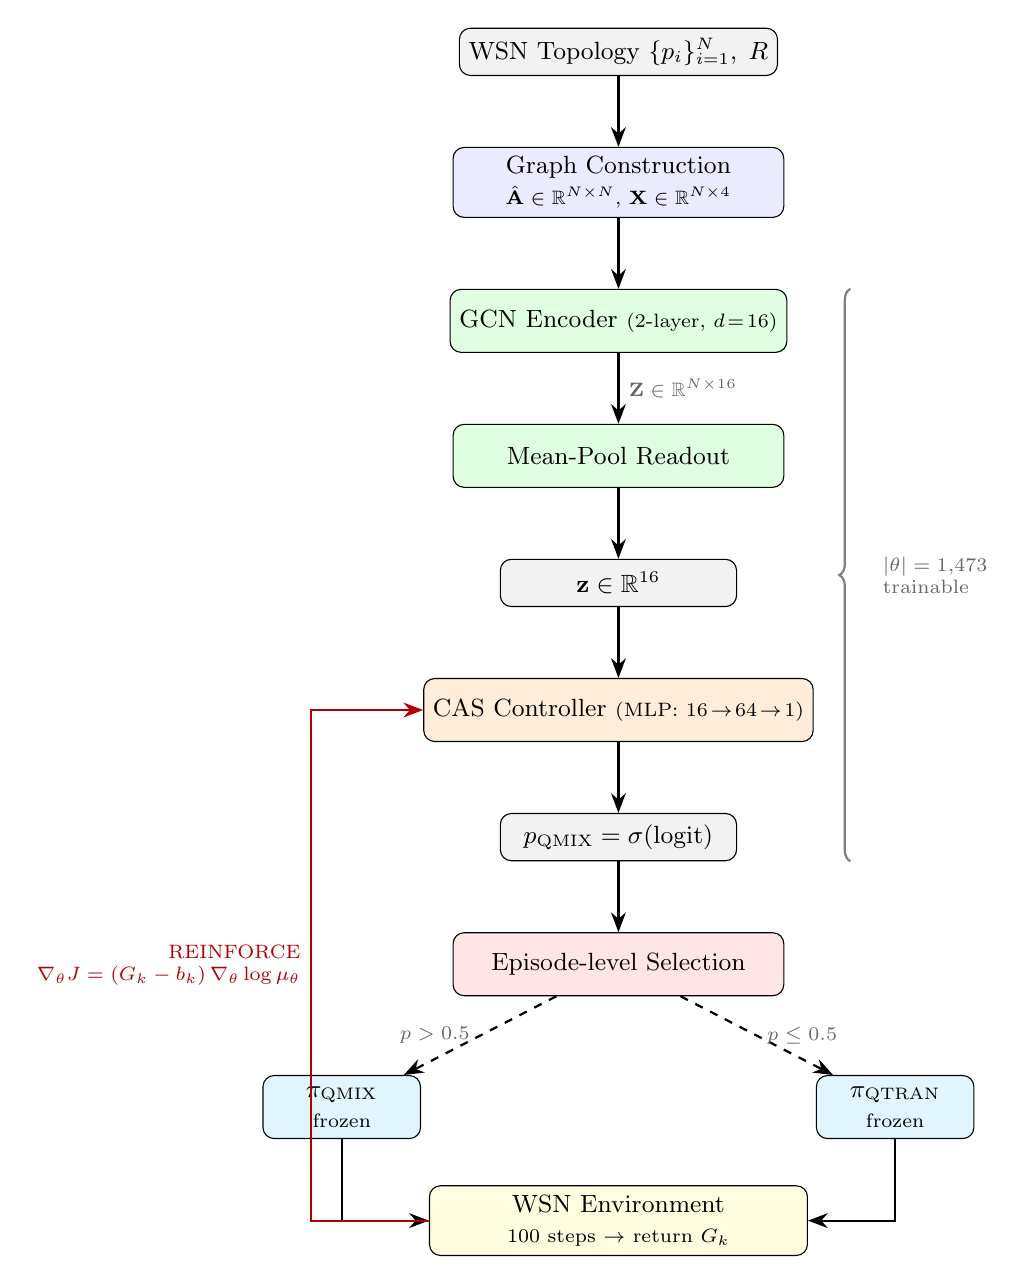
\begin{tikzpicture}[
    node distance=0.9cm,
    box/.style={draw, rounded corners, minimum height=0.8cm, minimum width=4.2cm, align=center, font=\small},
    data/.style={draw, rounded corners, minimum height=0.6cm, minimum width=3.0cm, align=center, fill=gray!10, font=\small},
    arrow/.style={-{Stealth[length=2.5mm]}, thick},
    dasharrow/.style={-{Stealth[length=2.5mm]}, thick, dashed},
    label/.style={font=\scriptsize, text=black!60},
]

% ===================== Top-down flow =====================

\node[data] (topo) {WSN Topology $\{p_i\}_{i=1}^N,\; R$};

\node[box, below=of topo, fill=blue!8] (graph) {Graph Construction\\{\scriptsize $\hat{\mathbf{A}} \in \mathbb{R}^{N \times N}$, $\mathbf{X} \in \mathbb{R}^{N \times 4}$}};

\node[box, below=of graph, fill=green!12] (gcn) {GCN Encoder {\scriptsize (2-layer, $d\!=\!16$)}};

\node[box, below=of gcn, fill=green!12] (pool) {Mean-Pool Readout};

\node[data, below=of pool] (embed) {$\mathbf{z} \in \mathbb{R}^{16}$};

\node[box, below=of embed, fill=orange!15] (cas) {CAS Controller {\scriptsize (MLP: $16 \!\to\! 64 \!\to\! 1$)}};

\node[data, below=of cas] (prob) {$p_{\text{QMIX}} = \sigma(\text{logit})$};

\node[box, below=of prob, fill=red!10] (decision) {Episode-level Selection};

% --- Experts side by side ---
\node[box, below left=1.0cm and 0.4cm of decision, fill=cyan!12, minimum width=2.0cm] (qmix) {$\pi_{\text{QMIX}}$\\{\scriptsize frozen}};
\node[box, below right=1.0cm and 0.4cm of decision, fill=cyan!12, minimum width=2.0cm] (qtran) {$\pi_{\text{QTRAN}}$\\{\scriptsize frozen}};

% --- Environment ---
\node[box, below=2.4cm of decision, fill=yellow!12, minimum width=4.8cm] (env) {WSN Environment\\{\scriptsize 100 steps $\to$ return $G_k$}};

% ===================== Arrows (top-down) =====================
\draw[arrow] (topo) -- (graph);
\draw[arrow] (graph) -- (gcn);
\draw[arrow] (gcn) -- node[right, label] {$\mathbf{Z} \in \mathbb{R}^{N \times 16}$} (pool);
\draw[arrow] (pool) -- (embed);
\draw[arrow] (embed) -- (cas);
\draw[arrow] (cas) -- (prob);
\draw[arrow] (prob) -- (decision);
\draw[dasharrow] (decision) -- node[left, label] {$p > 0.5$} (qmix);
\draw[dasharrow] (decision) -- node[right, label] {$p \leq 0.5$} (qtran);
\draw[arrow] (qmix) |- (env);
\draw[arrow] (qtran) |- (env);

% ===================== REINFORCE feedback =====================
\draw[arrow, red!70!black, thick]
    (env.west) -- ++(-1.5, 0) |- (cas.west)
    node[pos=0.25, left, font=\scriptsize, text=red!70!black, align=right]
    {REINFORCE\\$\nabla_\theta J = (G_k - b_k)\,\nabla_\theta \log \mu_\theta$};

% ===================== Brace: trainable params =====================
% Replace the brace with one spanning from GCN to CAS
\draw[decorate, decoration={brace, amplitude=4pt, mirror}, thick, black!50]
    let \p1=(gcn.north east), \p2=(prob.south east) in
    (\x1+0.8cm, \y1) -- (\x1+0.8cm, \y2)
    node[midway, right=8pt, font=\scriptsize, text=black!60, align=left] 
    {$|\theta| = 1{,}473$\\trainable};

\end{tikzpicture}
% }
\end{minipage}}
\captionof{figure}{GAPF architecture (CAS mode). Sensor positions and communication radius define a graph encoded by a two-layer GCN with mean-pool readout ($\mathbf{z} \in \mathbb{R}^{16}$). The CAS controller maps $\mathbf{z}$ to a selection probability $p_{\text{QMIX}}$. The chosen frozen expert executes the full episode. The return $G_k$ feeds back (red arrow) as a REINFORCE signal to update only the $1{,}473$ meta-controller parameters.}
\label{fig:gapf_architecture}
% \end{figure*}
\end{center}


\subsubsection{Training Procedure}
\label{sec:gapf_training}

GAPF is trained using the REINFORCE policy gradient algorithm~\cite{williams1992simple} with an exponential moving average (EMA) baseline to reduce variance.

\paragraph{Objective.}
Let $G_k$ denote the episodic return obtained by executing the selected expert $\pi_{a^{\text{meta}}_k}$ for the full episode~$k$. The policy gradient with respect to the meta-controller parameters $\theta$ is:
\begin{equation}
    \nabla_\theta J(\theta) = \mathbb{E}\!\left[\left(G_k - b_k\right) \nabla_\theta \log \mu_\theta\!\left(a^{\text{meta}}_k \mid \mathcal{G}_k\right)\right],
    \label{eq:reinforce}
\end{equation}
where $b_k$ is the EMA baseline updated as $b_{k+1} = \beta\, b_k + (1 - \beta)\, G_k$ with $\beta = 0.95$.

\paragraph{Log-probability.}
Since $a^{\text{meta}} \in \{\text{QMIX}, \text{QTRAN}\}$ is a Bernoulli variable:
\begin{equation}
    \log \mu_\theta\!\left(a^{\text{meta}} \mid \mathcal{G}\right) = 
    \begin{cases}
        \log p_{\text{QMIX}} & \text{if } a^{\text{meta}} = \text{QMIX}, \\
        \log(1 - p_{\text{QMIX}}) & \text{if } a^{\text{meta}} = \text{QTRAN}.
    \end{cases}
    \label{eq:log_prob}
\end{equation}

\paragraph{Update rule.}
At each training episode, the parameters are updated via:
\begin{equation}
    \theta \leftarrow \theta + \alpha \cdot (G_k - b_k) \cdot \nabla_\theta \log \mu_\theta(a^{\text{meta}}_k \mid \mathcal{G}_k),
    \label{eq:update}
\end{equation}
with learning rate $\alpha = 3 \times 10^{-3}$ and gradient clipping $\|\nabla_\theta\|_2 \leq 1.0$.

The complete training procedure is summarised in Algorithm~\ref{alg:gapf_training}.

\begin{algorithm}[H]
\caption{GAPF Training (CAS Mode)}
\label{alg:gapf_training}
\scalebox{0.75}{\begin{minipage}{\linewidth}
\begin{algorithmic}[1]
\REQUIRE Pre-trained frozen experts $\pi_{\text{QMIX}}$, $\pi_{\text{QTRAN}}$; WSN environment; number of training episodes $K$
\ENSURE Trained meta-controller parameters $\theta$
\STATE Initialise $\theta$ randomly; $b \leftarrow \text{None}$
\FOR{$k = 1, \dots, K$}
    \STATE Reset environment; observe topology $\mathcal{G}_k$
    \STATE Construct $\hat{\mathbf{A}}_k$ (Eq.~\ref{eq:norm_adj}) and $\mathbf{X}_k$ (Eq.~\ref{eq:node_features})
    \STATE $\mathbf{z}_k \leftarrow \text{GCN}(\mathbf{X}_k, \hat{\mathbf{A}}_k)$ \hfill \COMMENT{Graph embedding (Eqs.~\ref{eq:gcn_layer1}--\ref{eq:readout})}
    \STATE $p_{\text{QMIX}} \leftarrow \text{CAS}(\mathbf{z}_k)$ \hfill \COMMENT{Selection probability (Eq.~\ref{eq:cas_controller})}
    \STATE Sample $a^{\text{meta}}_k \sim \text{Bernoulli}(p_{\text{QMIX}})$
    \STATE Execute $\pi_{a^{\text{meta}}_k}$ for the full episode; collect return $G_k$
    \IF{$b = \text{None}$}
        \STATE $b \leftarrow G_k$
    \ENDIF
    \STATE $\delta_k \leftarrow G_k - b$ \hfill \COMMENT{Advantage estimate}
    \STATE $b \leftarrow 0.95 \cdot b + 0.05 \cdot G_k$ \hfill \COMMENT{Update EMA baseline}
    \IF{$|\delta_k| > 10^{-8}$}
        \STATE $\mathcal{L} \leftarrow -\delta_k \cdot \log \mu_\theta(a^{\text{meta}}_k \mid \mathcal{G}_k)$
        \STATE $\theta \leftarrow \theta - \alpha \cdot \text{clip}(\nabla_\theta \mathcal{L},\; 1.0)$ \hfill \COMMENT{Adam update}
    \ENDIF
\ENDFOR
\end{algorithmic}
\end{minipage}}
\end{algorithm}

\subsubsection{Design Rationale}
\label{sec:gapf_rationale}

Several design choices distinguish GAPF from standard ensemble methods:

\begin{enumerate}[leftmargin=*]
    \item \textbf{Topology awareness.} GAPF uses a GCN to encode the spatial graph of the sensor network. This allows the meta-controller to learn that certain topologies (e.g., sparse, disconnected networks) may favour one expert over another.
    
    \item \textbf{Episode-level granularity.} In CAS mode, the selection is made \emph{once per episode}, not at every timestep. This avoids the instability of switching experts mid-episode, where different experts may have incompatible hidden state dynamics in their GRU-based agents.
    
    \item \textbf{Minimal overhead.} With only $1{,}473$ trainable parameters (Table~\ref{tab:hyperparameters}), GAPF adds negligible computation compared to the underlying experts ($38{,}983$ parameters each). The GCN encoding is performed once per episode, and the CAS decision is a single forward pass through a two-layer MLP.
    
    \item \textbf{Frozen experts.} The pre-trained QMIX and QTRAN policies are \emph{not fine-tuned} during GAPF training. This preserves their independently validated performance and reduces the optimisation landscape to only $1{,}473$ dimensions, enabling fast convergence with REINFORCE despite its high variance.
    
    \item \textbf{Deployment feasibility.} The per-agent routing model (GRU with $38{,}983$ parameters $\approx 38$\,KB in int8 quantisation) fits within the RAM constraints of typical WSN microcontrollers (e.g., nRF52840: 256\,KB RAM, ESP32: 520\,KB RAM), enabling on-device inference without an edge server.
\end{enumerate}


\begin{center}
\captionof{table}{Training Hyperparameters for QMIX, QTRAN, and GAPF}
\label{tab:hyperparameters}
\resizebox{\textwidth}{!}{
\begin{tabular}{llccc}
\toprule
\textbf{Category} & \textbf{Parameter} & \textbf{QMIX} & \textbf{QTRAN} & \textbf{GAPF} \\
\midrule
\multirow{5}{*}{Optimization}
 & Optimizer           & Adam     & RMSprop  & Adam     \\
 & Learning rate       & 0.0003   & 0.0003   & 0.003    \\
 & Gradient clip norm  & 10       & 10       & 1.0      \\
 & Discount $\gamma$   & 0.99     & 0.99     & ---      \\
 & Reward scale        & 0.01     & 0.01     & ---      \\
\midrule
\multirow{4}{*}{Exploration}
 & Strategy                    & $\varepsilon$-greedy & $\varepsilon$-greedy & REINFORCE \\
 & $\varepsilon_{\text{start}}$  & 0.5    & 0.5    & ---  \\
 & $\varepsilon_{\text{end}}$    & 0.01   & 0.01   & ---  \\
 & Anneal timesteps            & 150\,000 & 150\,000 & --- \\
\midrule
\multirow{5}{*}{Architecture}
 & Agent network        & GRU (64) & GRU (64) & GCN + MLP \\
 & RNN hidden dim       & 64       & 64       & ---       \\
 & Mixing embed dim     & 64       & 64       & ---       \\
 & GNN embed dim        & ---      & ---      & 16        \\
 & Meta-controller hidden & ---    & ---      & 64        \\
\midrule
\multirow{4}{*}{Training}
 & Total timesteps $t_{\max}$   & 200\,000 & 200\,000 & ---       \\
 & Training episodes            & $\sim$2\,000 & $\sim$2\,000 & 2\,000 \\
 & Batch size (episodes)        & 32       & 32       & 1 (on-policy) \\
 & Replay buffer size           & 15\,000  & 15\,000  & ---       \\
\midrule
\multirow{3}{*}{Target / Baseline}
 & Target update        & Hard, every 30 ep. & Hard, every 30 ep. & ---            \\
 & Double Q-learning    & Yes      & Yes      & ---            \\
 & Baseline EMA $\beta$ & ---      & ---      & 0.95           \\
\midrule
\multirow{3}{*}{QTRAN-specific}
 & Optimality loss weight $\lambda_{\text{opt}}$     & --- & 1.0  & --- \\
 & Non-optimality loss weight $\lambda_{\text{nopt}}$ & --- & 0.1  & --- \\
 & Loss function        & Huber ($\beta$=10) & TD + constraints & Policy gradient \\
\midrule
\multirow{2}{*}{Evaluation}
 & Test episodes        & 1\,000   & 1\,000   & 1\,000   \\
 & Eval $\varepsilon$   & 0.01     & 0.01     & ---      \\
\bottomrule
\end{tabular}
}
\end{center}

\end{reply}
\end{mdframed}

\begin{point}
Second, the algorithmic details are presented only at a high level; more formal pseudocode or implementation details would strengthen reproducibility.
\end{point}

\begin{mdframed}[style=Resp]
\begin{reply}\label{1:2}
As suggested, we have incorporated a more formal pseudocode or implementation details. It is summarized at the \textbf{\textcolor{blue}{Section III.E, Algorithm 1 of the revised manuscript}}. The graph construction procedure is detailed in Algorithm~\ref{alg:graph_construction}.

\begin{algorithm}[H]
\caption{Graph Construction and Feature Extraction}
\label{alg:graph_construction}
\begin{algorithmic}[1]
\REQUIRE Sensor positions $\{p_i\}_{i=1}^N \subset \mathbb{R}^2$, communication radius $R$, base station position $p_{\text{BS}}$, field size $L$
\ENSURE Normalised adjacency $\hat{\mathbf{A}} \in \mathbb{R}^{N \times N}$, node features $\mathbf{X} \in \mathbb{R}^{N \times 4}$
\STATE \textbf{// Adjacency matrix}
\FOR{$i = 1, \dots, N$}
    \FOR{$j = 1, \dots, N$}
        \STATE $A_{ij} \leftarrow \mathbf{1}\!\left[\|p_i - p_j\|_2 \leq R\right] \cdot \mathbf{1}[i \neq j]$
    \ENDFOR
\ENDFOR
\STATE \textbf{// Symmetric normalisation~\cite{kipf2017semi}}
\STATE $\tilde{\mathbf{A}} \leftarrow \mathbf{A} + \mathbf{I}_N$
\STATE $\tilde{D}_{ii} \leftarrow \sum_j \tilde{A}_{ij}$ \hfill $\triangleright$ Degree of node $i$ in self-looped graph
\STATE $\hat{\mathbf{A}} \leftarrow \tilde{\mathbf{D}}^{-1/2}\,\tilde{\mathbf{A}}\,\tilde{\mathbf{D}}^{-1/2}$
\STATE \textbf{// Node features (all normalised to $[0,1]$)}
\FOR{$i = 1, \dots, N$}
    \STATE $d_i^{\text{BS}} \leftarrow \|p_i - p_{\text{BS}}\|_2$ \hfill $\triangleright$ Distance to base station
    \STATE $\deg(i) \leftarrow \sum_j A_{ij}$ \hfill $\triangleright$ Degree in original graph
    \STATE $\mathbf{x}_i \leftarrow \left[\;\dfrac{p_i^{(x)}}{L},\;\; \dfrac{p_i^{(y)}}{L},\;\; \dfrac{d_i^{\text{BS}}}{\max_j d_j^{\text{BS}}},\;\; \dfrac{\deg(i)}{\max_j \deg(j)}\;\right]^\top$
\ENDFOR
\STATE $\mathbf{X} \leftarrow [\mathbf{x}_1, \dots, \mathbf{x}_N]^\top$
\RETURN $\hat{\mathbf{A}},\; \mathbf{X}$
\end{algorithmic}
\end{algorithm}

The complete episode execution, including the GCN forward pass, CAS decision, 
and step-by-step expert rollout, is formalised in Algorithm~\ref{alg:gapf_episode}. 

\begin{algorithm}[H]
\caption{GAPF Episode Execution (CAS Mode)}
\label{alg:gapf_episode}
\begin{algorithmic}[1]
\REQUIRE Environment $\mathcal{M}$, frozen experts $\pi_{\text{QMIX}}$, $\pi_{\text{QTRAN}}$ (each a BasicMAC with GRU-64 agent), GAPF model $\mu_\theta$, training flag
\ENSURE Episode return $G_k$, log-probability $\ell_k$, metrics
\STATE $\mathcal{M}.\text{reset}()$; \; read sensor positions $\{p_i\}$, radius $R$
\STATE $\hat{\mathbf{A}},\, \mathbf{X} \leftarrow \textsc{GraphConstruction}(\{p_i\}, R)$ \hfill $\triangleright$ Alg.~\ref{alg:graph_construction}
\STATE \textbf{// GCN encoding (once per episode)}
\STATE $\mathbf{H}^{(1)} \leftarrow \text{ReLU}(\hat{\mathbf{A}}\,\mathbf{X}\,\mathbf{W}_1)$ \hfill $\triangleright$ $\mathbf{W}_1 \in \mathbb{R}^{4 \times 16}$
\STATE $\mathbf{Z} \leftarrow \hat{\mathbf{A}}\,\mathbf{H}^{(1)}\,\mathbf{W}_2$ \hfill $\triangleright$ $\mathbf{W}_2 \in \mathbb{R}^{16 \times 16}$
\STATE $\mathbf{z} \leftarrow \frac{1}{N}\sum_{i=1}^{N} \mathbf{Z}_{i,:}$ \hfill $\triangleright$ Mean-pool readout, $\mathbf{z} \in \mathbb{R}^{16}$
\STATE \textbf{// CAS decision}
\STATE $\text{logit} \leftarrow \mathbf{w}_2^\top \,\text{ReLU}(\mathbf{W}_c\,\mathbf{z} + \mathbf{b}_c) + b_2$ \hfill $\triangleright$ $\mathbf{W}_c \!\in\! \mathbb{R}^{64 \times 16}$
\STATE $p_{\text{QMIX}} \leftarrow \sigma(\text{logit})$
\IF{training}
    \STATE Sample $u \sim \text{Uniform}(0,1)$
    \STATE $a^{\text{meta}} \leftarrow \mathbf{1}[u < p_{\text{QMIX}}]$ \hfill $\triangleright$ $1$: QMIX, $0$: QTRAN
    \STATE $\ell_k \leftarrow a^{\text{meta}} \cdot \log p_{\text{QMIX}} + (1 - a^{\text{meta}}) \cdot \log(1 - p_{\text{QMIX}})$
\ELSE
    \STATE $a^{\text{meta}} \leftarrow \mathbf{1}[p_{\text{QMIX}} > 0.5]$ \hfill $\triangleright$ Greedy selection
    \STATE $\ell_k \leftarrow \text{None}$
\ENDIF
\STATE $\pi \leftarrow \pi_{\text{QMIX}}$ \textbf{if} $a^{\text{meta}} = 1$ \textbf{else} $\pi_{\text{QTRAN}}$
\STATE Initialise GRU hidden states: $h_i^{(0)} \leftarrow \mathbf{0} \in \mathbb{R}^{64}$, $\forall i \in \{1,\dots,N\}$
\STATE $G_k \leftarrow 0$
\STATE \textbf{// Execute selected expert for the full episode}
\FOR{$t = 0, \dots, T_{\max} - 1$}
    \STATE $o_i^{(t)} \leftarrow \mathcal{M}.\text{get\_obs}(i)$, $\forall i$ \hfill $\triangleright$ $o_i \in \mathbb{R}^{5}$
    \STATE $m_i^{(t)} \leftarrow \mathcal{M}.\text{get\_avail\_actions}(i)$, $\forall i$ \hfill $\triangleright$ $m_i \in \{0,1\}^{n_{\text{act}}}$
    \FOR{$i = 1, \dots, N$}
        \STATE $\tilde{o}_i^{(t)} \leftarrow [o_i^{(t)};\; \text{onehot}(a_i^{(t-1)});\; \text{onehot}(i)]$ \hfill $\triangleright$ Input: $\mathbb{R}^{146}$
        \STATE $h_i^{(t)} \leftarrow \text{GRU}(\tilde{o}_i^{(t)},\, h_i^{(t-1)})$ \hfill $\triangleright$ Hidden: $\mathbb{R}^{64}$
        \STATE $Q_i^{(t)} \leftarrow \mathbf{W}_q\, h_i^{(t)} + \mathbf{b}_q$ \hfill $\triangleright$ Q-values: $\mathbb{R}^{n_{\text{act}}}$
        \STATE $Q_i^{(t)}[m_i^{(t)} = 0] \leftarrow -\infty$ \hfill $\triangleright$ Mask unavailable actions
        \STATE $a_i^{(t)} \leftarrow \arg\max Q_i^{(t)}$ \hfill $\triangleright$ Greedy action
    \ENDFOR
    \STATE $r^{(t)},\, \text{done} \leftarrow \mathcal{M}.\text{step}(\{a_i^{(t)}\}_{i=1}^N)$
    \STATE $G_k \leftarrow G_k + r^{(t)}$
    \IF{done}
        \STATE \textbf{break}
    \ENDIF
\ENDFOR
\RETURN $G_k,\; \ell_k,\; \text{metrics}$
\end{algorithmic}
\end{algorithm}

The outer REINFORCE training loop is presented in Algorithm~\ref{alg:gapf_training}.

\begin{algorithm}[H]
\caption{GAPF Training (CAS Mode)}
\label{alg:gapf_training}
\begin{algorithmic}[1]
\REQUIRE Pre-trained frozen experts $\pi_{\text{QMIX}}$, $\pi_{\text{QTRAN}}$; WSN environment $\mathcal{M}$; training episodes $K$; learning rate $\alpha = 3 \times 10^{-3}$; baseline decay $\beta = 0.95$; gradient clip norm $c = 1.0$
\ENSURE Trained meta-controller parameters $\theta$
\STATE Initialise $\theta$ randomly (Xavier uniform)
\STATE Initialise Adam optimiser with learning rate $\alpha$
\STATE $b \leftarrow \text{None}$ \hfill $\triangleright$ EMA baseline
\FOR{$k = 1, \dots, K$}
    \STATE \textbf{// Rollout}
    \STATE $G_k,\, \ell_k,\, \_ \leftarrow \textsc{GAPFEpisode}(\mathcal{M}, \pi_{\text{QMIX}}, \pi_{\text{QTRAN}}, \mu_\theta, \text{training=True})$
    \STATE \hfill $\triangleright$ Alg.~\ref{alg:gapf_episode}
    \STATE \textbf{// Baseline update}
    \IF{$b = \text{None}$}
        \STATE $b \leftarrow G_k$ \hfill $\triangleright$ Initialise from first episode
    \ENDIF
    \STATE $\delta_k \leftarrow G_k - b$ \hfill $\triangleright$ Advantage estimate
    \STATE $b \leftarrow \beta \cdot b + (1 - \beta) \cdot G_k$ \hfill $\triangleright$ Update EMA baseline
    \STATE \textbf{// Policy gradient update}
    \IF{$|\delta_k| > 10^{-8}$}
        \STATE $\mathcal{L} \leftarrow -\delta_k \cdot \ell_k$ \hfill $\triangleright$ REINFORCE loss
        \STATE $\theta \leftarrow \theta - \alpha \cdot \text{Adam}\!\left(\text{clip}\!\left(\nabla_\theta \mathcal{L},\; c\right)\right)$
    \ENDIF
\ENDFOR
\RETURN $\theta$
\end{algorithmic}
\end{algorithm}
 
\end{reply}
\end{mdframed}

\begin{point}
Third, while the novelty is partially clear, the contribution can appear incremental, as much of the performance gain comes from the improved reward modeling rather than a fundamentally new algorithmic design.

\end{point}

\begin{mdframed}[style=Resp]
\begin{reply}
Following a thorough review of our manuscript, we have developed a substantially revised algorithm, as detailed in our responses to the preceding comments. In addition, the reward function has been restructured as follows. It is summarized at the (\textbf{\textcolor{blue}{Section III.D of the revised manuscript}}):

\subsection{Reward Scalarization via Monotonic Q$\cdot$K Attention Network}
\label{sec:reward_scalarization}

Multi-objective reward design is a fundamental challenge in cooperative MARL for WSN routing: agents must simultaneously optimize energy efficiency, energy balance, directional progress toward the base station, and load distribution across nodes. Naïve approaches—such as fixed linear combinations of objectives—require manual weight tuning that does not generalize across topologies and traffic conditions. We introduce a \emph{Monotonic Q$\cdot$K Attention Network} that \textbf{(i)} learns objective importance weights via a scaled dot-product attention mechanism, \textbf{(ii)} guarantees monotonicity so that Pareto-improving actions are never penalized, and \textbf{(iii)} adapts online through an Evolution Strategies (ES) meta-learning loop.

\subsubsection{Individual Reward Objectives}
\label{sec:individual_rewards}

At each time step $t$, when sensor $i$ relays its packets to a neighbor $j$, the environment computes a four-dimensional reward vector $\mathbf{r}_i^{(t)} = [r_1, r_2, r_3, r_4] \in [0,1]^4$, where each component captures a distinct routing objective:

\paragraph{Directional Progress ($r_1$: Angle to BS).}
Measures the alignment between the relay direction $\overrightarrow{ij}$ and the ideal direction toward the base station $\overrightarrow{i\,\mathrm{BS}}$:
\begin{equation}
    r_1 = 1 - \frac{|\theta_{ij}|}{\pi}, \qquad \theta_{ij} = \arccos\!\left(\frac{\overrightarrow{ij} \cdot \overrightarrow{i\,\mathrm{BS}}}{\|\overrightarrow{ij}\|\;\|\overrightarrow{i\,\mathrm{BS}}\|}\right)
    \label{eq:reward_angle}
\end{equation}
When $j$ lies in the exact direction of the BS, $r_1 = 1$; when $j$ is in the opposite direction, $r_1 = 0$.

\paragraph{Energy Efficiency ($r_2$: Transmission Cost).}
Penalizes high energy consumption for the relay hop:
\begin{equation}
    r_2 = 1 - \frac{E_{\mathrm{tx}}(p_i, d_{ij}) + E_{\mathrm{rx}}(p_i)}{E_{\mathrm{tx}}^{\max} + E_{\mathrm{rx}}^{\max}}
    \label{eq:reward_energy}
\end{equation}
where $E_{\mathrm{tx}}(p_i, d_{ij})$ and $E_{\mathrm{rx}}(p_i)$ are the transmission and reception energies for $p_i$ packets over distance $d_{ij}$, normalized by the worst-case energies $E_{\mathrm{tx}}^{\max} = E_{\mathrm{tx}}(N \cdot p_0, R)$ and $E_{\mathrm{rx}}^{\max} = E_{\mathrm{rx}}(N \cdot p_0)$, with $N$ the number of sensors, $p_0$ the initial packet count, and $R$ the coverage radius.

\paragraph{Energy Balance ($r_3$: Remaining Energy Dispersion).}
Encourages uniform energy depletion across the network to maximize network lifetime:
\begin{equation}
    r_3 = 1 - \frac{\sigma(\mathbf{e}_{\mathrm{rem}})}{E_0 / 2}
    \label{eq:reward_dispersion}
\end{equation}
where $\sigma(\mathbf{e}_{\mathrm{rem}})$ is the standard deviation of remaining energies across all sensors and $E_0 / 2$ is the theoretical maximum standard deviation (achieved when half the sensors are fully charged and half are depleted).

\paragraph{Load Balancing ($r_4$: Receiver Packet Buffer).}
Discourages routing through already overloaded relay nodes:
\begin{equation}
    r_4 = 1 - \frac{p_j}{N \cdot p_0}
    \label{eq:reward_packets}
\end{equation}
where $p_j$ is the current packet count at the receiver node $j$.

All four components are clipped to $[0,1]$, ensuring a well-defined input domain for the scalarization network.

\subsubsection{Monotonic Q$\cdot$K Attention Architecture}
\label{sec:monotonic_architecture}

The scalarization function $f_\phi: [0,1]^4 \to \mathbb{R}$ maps the individual reward vector $\mathbf{r}$ to a scalar reward. It is composed of two stages: an input-independent attention weighting and a monotonic feed-forward network.

\paragraph{Stage 1: Scaled Dot-Product Attention over Objectives.}
We define a learnable query vector $\mathbf{q} \in \mathbb{R}^d$ and a key matrix $\mathbf{K} = [\mathbf{k}_1, \mathbf{k}_2, \mathbf{k}_3, \mathbf{k}_4]^\top \in \mathbb{R}^{4 \times d}$, where $d = 16$ is the embedding dimension. The attention weights are:
\begin{equation}
    \alpha_i = \frac{\exp(\mathbf{k}_i^\top \mathbf{q} / \sqrt{d})}{\sum_{j=1}^{4} \exp(\mathbf{k}_j^\top \mathbf{q} / \sqrt{d})}, \qquad i \in \{1,2,3,4\}
    \label{eq:attention_weights}
\end{equation}
The weighted input is then $\mathbf{r}' = \boldsymbol{\alpha} \odot \mathbf{r}$, where $\odot$ denotes element-wise multiplication.

\begin{remark}[Input-Independence]
\label{rem:input_independence}
Crucially, the attention weights $\boldsymbol{\alpha}$ depend \emph{only} on the learnable parameters $(\mathbf{q}, \mathbf{K})$ and \emph{not} on the input $\mathbf{r}$. Since $\alpha_i > 0$ for all $i$ (due to the softmax), the weighting $\mathbf{r}' = \boldsymbol{\alpha} \odot \mathbf{r}$ preserves the partial ordering: $\mathbf{r}^{(1)} \leq \mathbf{r}^{(2)}$ component-wise implies $\mathbf{r}'^{(1)} \leq \mathbf{r}'^{(2)}$.
\end{remark}

\paragraph{Stage 2: Monotonic Feed-Forward Network.}
The weighted input $\mathbf{r}'$ is passed through a monotonic neural network $g_\psi: \mathbb{R}^4 \to \mathbb{R}$:
\begin{equation}
    g_\psi(\mathbf{r}') = \mathbf{W}_3\;\sigma\!\left(\mathbf{W}_2\;\sigma\!\left(\mathbf{W}_1\;\mathbf{r}' + \mathbf{b}_1\right) + \mathbf{b}_2\right) + b_3
    \label{eq:monotonic_net}
\end{equation}
where $\sigma(\cdot) = \log(1 + e^{(\cdot)})$ is the softplus activation and each weight matrix is constrained to be non-negative:
\begin{equation}
    \mathbf{W}_\ell = \mathrm{softplus}(\mathbf{W}_\ell^{\mathrm{raw}}), \qquad \mathbf{W}_\ell \geq 0
    \label{eq:weight_constraint}
\end{equation}
The layer dimensions are $4 \to 16 \to 16 \to 1$.

\begin{theorem}[Monotonicity Guarantee]
\label{thm:monotonicity}
For any $\mathbf{r}^{(1)}, \mathbf{r}^{(2)} \in [0,1]^4$ with $\mathbf{r}^{(1)} \leq \mathbf{r}^{(2)}$ component-wise, the network output satisfies $f_\phi(\mathbf{r}^{(1)}) \leq f_\phi(\mathbf{r}^{(2)})$.
\end{theorem}

\begin{proof}
Since $\alpha_i > 0$ for all $i$ (Remark~\ref{rem:input_independence}), $\mathbf{r}^{(1)} \leq \mathbf{r}^{(2)}$ implies $\boldsymbol{\alpha} \odot \mathbf{r}^{(1)} \leq \boldsymbol{\alpha} \odot \mathbf{r}^{(2)}$. For each monotonic layer, the Jacobian satisfies $\partial g / \partial r'_i = \sigma'(\cdot) \cdot W_i \geq 0$, since the softplus derivative $\sigma'(x) = (1 + e^{-x})^{-1} \in (0,1)$ and $W_i \geq 0$. By the chain rule applied over all layers, the composition $f_\phi = g_\psi \circ (\boldsymbol{\alpha} \odot \cdot)$ is monotonically non-decreasing in each input component.
\end{proof}

The monotonicity property is essential: it ensures that a Pareto-dominating action (\emph{i.e.}, one that improves every objective simultaneously) always receives a higher scalar reward, preventing pathological reward shaping.

\paragraph{Reward Centering.}
To improve the signal-to-noise ratio, the network output is centered by subtracting a baseline computed at the zero input:
\begin{equation}
    \hat{f}_\phi(\mathbf{r}) = f_\phi(\mathbf{r}) - f_\phi(\mathbf{0})
    \label{eq:reward_centering}
\end{equation}
The baseline $f_\phi(\mathbf{0})$ is recomputed once per episode after the ES perturbation (Section~\ref{sec:es_learning}).

\subsubsection{Composite Step Reward}
\label{sec:composite_reward}

The final scalar reward for sensor $i$ at step $t$ depends on its action type:

\paragraph{Delivery to Base Station.}
When sensor $i$ successfully delivers packets directly to the BS:
\begin{equation}
    r_i^{(t)} = \beta_{\mathrm{del}} \cdot p_i
    \label{eq:delivery_reward}
\end{equation}
where $\beta_{\mathrm{del}} = 100$ is the delivery bonus and $p_i$ is the number of packets delivered. This strong signal is \emph{not} passed through the attention network—delivery is the terminal objective and needs no scalarization.

\paragraph{Relay to Neighbor.}
When sensor $i$ relays packets to a neighbor $j \neq \mathrm{BS}$:
\begin{equation}
    r_i^{(t)} = \underbrace{\hat{f}_\phi(\mathbf{r}_i^{(t)}) \cdot \lambda_{\mathrm{attn}}}_{\text{attention-scalarized reward}} \;+\; \underbrace{\frac{d(i, \mathrm{BS}) - d(j, \mathrm{BS})}{R} \cdot 0.5}_{\text{progress shaping}}
    \label{eq:relay_reward}
\end{equation}
where $\lambda_{\mathrm{attn}} = 0.01$ scales the attention output to prevent relay-loop farming (agents exploiting relay rewards without progressing toward the BS), and the progress shaping term rewards relays that reduce the packet's distance to the BS.

\paragraph{Invalid Actions.}
Self-loops receive $r_i = -0.1$; out-of-range transmissions receive $r_i = -0.1$; failed transmissions due to insufficient energy receive $r_i = -0.5$; inactive sensors (depleted energy or no packets) receive $r_i = 0$.

\subsubsection{Evolution Strategies Meta-Learning}
\label{sec:es_learning}

The attention network parameters $\phi = (\mathbf{q}, \mathbf{K}, \{\mathbf{W}_\ell^{\mathrm{raw}}, \mathbf{b}_\ell\}_\ell)$ are trained via an outer-loop Evolution Strategies (ES)~\cite{salimans2017evolution} procedure that does not require differentiating through the RL episode:

\paragraph{Meta-Objective.}
At the end of each episode, a meta-objective $J$ evaluates the \emph{true} network-level goals:
\begin{equation}
    J = \underbrace{\left(1 - \frac{\sum_{i=1}^{N}(E_0 - e_i^{\mathrm{rem}})}{N \cdot E_0}\right)}_{\text{energy efficiency}} + \underbrace{\left(1 - \frac{\sigma(\mathbf{e}_{\mathrm{rem}})}{E_0 / 2}\right)}_{\text{energy balance}}, \qquad J \in [0, 2]
    \label{eq:meta_objective}
\end{equation}
where $e_i^{\mathrm{rem}}$ is the remaining energy of sensor $i$ at episode end. This meta-objective directly measures the network-level outcomes we care about, independently of the proxy rewards used during the episode.

\paragraph{ES Update Procedure.}
The three-step procedure operates at the episode granularity:

\begin{enumerate}
    \item \textbf{Perturbation (before episode):} Sample $\boldsymbol{\varepsilon} \sim \mathcal{N}(\mathbf{0}, \mathbf{I})$ for each parameter and apply $\phi' = \phi + \sigma_{\mathrm{ES}} \boldsymbol{\varepsilon}$, where $\sigma_{\mathrm{ES}} = 0.01$.
    \item \textbf{Episode execution:} Run the full episode with perturbed parameters $\phi'$, compute $J(\phi')$.
    \item \textbf{Update (after episode):} Compute the advantage $A = J(\phi') - \bar{J}$, where $\bar{J}$ is an exponential moving average baseline with decay $\beta = 0.9$. Restore original parameters and update:
    \begin{equation}
        \phi \leftarrow \phi + \eta_{\mathrm{ES}} \cdot A \cdot \boldsymbol{\varepsilon}, \qquad \eta_{\mathrm{ES}} = 0.01
        \label{eq:es_update}
    \end{equation}
    The update is skipped when $|A| < 0.01$ to reduce noise.
\end{enumerate}

This bi-level optimization decouples the inner-loop RL training (which maximizes cumulative scalar rewards) from the outer-loop reward shaping (which adapts the scalarization to maximize the true network-level objectives).

\paragraph{Initialization Bias.}
The key embeddings are initialized with a domain-informed prior: energy ($\mathbf{k}_2$) and dispersion ($\mathbf{k}_3$) keys are initialized close to $\mathbf{q}$ (yielding higher initial attention), while angle ($\mathbf{k}_1$) and packet load ($\mathbf{k}_4$) keys are initialized randomly. This accelerates convergence by encoding the domain knowledge that energy-related objectives are typically more important in WSN routing, while still allowing the ES procedure to discover the optimal weighting.

\paragraph{Attention Interpretability.}
The learned attention weights $\boldsymbol{\alpha}$ provide direct interpretability: at any point during training, the relative importance assigned to each objective can be inspected. For example, if $\alpha_2 \gg \alpha_1$, the network has learned that energy efficiency is more critical than directional progress for the current scenario. This is reported in the training logs via the \texttt{get\_interpretable\_summary()} method.


\end{reply}
\end{mdframed}


\begin{point}
Fourth, the paper does not train QMIX and QTRAN simultaneously, but instead separately and then dynamically selects between them, which should be clarified more explicitly.

\end{point}

\begin{mdframed}[style=Resp]
\begin{reply}
We thank the reviewers for their feedback, and we have clarified this point as follows: QMIX and QTRAN are trained independently as separate expert policies. Their parameters are then frozen, and only the lightweight GAPF meta-controller (~1,473 parameters) is trained to dynamically select between these frozen experts based on the network topology (\textbf{\textcolor{blue}{Just after Table III of the revised manuscript}}).

\end{reply}
\end{mdframed}

\begin{point}
Fifth, the approach is validated only in simulation, and the computational feasibility on real, resource-constrained WSN nodes remains uncertain.

\end{point}

\begin{mdframed}[style=Resp]
\begin{reply}\label{pratical_feas5}
We thank the reviewer for this important concern. We address it in two parts: (A) the computational feasibility evidence already present in our framework, and (B) the concrete deployment path enabled by the Centralized Training, Decentralized Execution (CTDE) paradigm.

(A) Computational Feasibility Analysis

Our framework includes a dedicated inference benchmarking tool that measures, for each algorithm: inference latency distribution (p50/p95/p99 and jitter), averaged over 30 iterations with 3 warmup passes; peak memory footprint (via tracemalloc); analytical MACs/FLOPs counts computed from the network architecture; and estimated energy per inference (µJ), calibrated to a user-specified device power budget (W).

Additionally, every episode during both training and evaluation automatically records wall-clock step time (mean, p95, p99), episode time, and peak RSS memory. These metrics are saved as versioned .npy arrays and summarized into PASS/FAIL feasibility tables against real-time deadline budgets (e.g., 10 ms and 50 ms per decision step, 1024 MB peak memory). Table X of the revised manuscript reports these results.

(B) Deployment Path Under the CTDE Paradigm

A critical point is that our system follows the Centralized Training, Decentralized Execution (CTDE) paradigm, which fundamentally separates the training infrastructure from the deployed system. At inference, each sensor node executes only its local agent network: a single-layer GRU with architecture input(5) → Linear(5,64) → ReLU → GRUCell(64,64) → Linear(64,31) → argmax. The QMIX/QTRAN mixers, the Monotonic Q·K Attention reward network, and the Evolution Strategies meta-learning loop are all training-only components that are never deployed.

The GAPF meta-controller runs only at the sink/gateway node (typically a Raspberry Pi or similar edge device), and only once per episode — a single GCN forward pass over 1,473 parameters. Its overhead on the sensor network is zero.

After training completes on a standard server: (1) the trained agent weights are extracted from the PyTorch checkpoint as flat float arrays; (2) the GRU forward pass is implemented in ~100 lines of C (or via TFLite Micro / microTVM); (3) the weight arrays are stored in flash memory (~100 KB) on each sensor's microcontroller (e.g., ARM Cortex-M4: STM32L4 with 1 MB flash, 256 KB SRAM; or Nordic nRF52840 with 1 MB flash, 256 KB RAM); (4) at runtime, each sensor performs one GRU forward pass per routing step, selecting the next-hop neighbor via argmax over Q-values.

This deployment model is identical to that of all CTDE-based MARL methods (QMIX, QTRAN, MAPPO). The per-sensor agent complexity is determined by the agent network architecture shared across all these methods, not by our GAPF contribution. GAPF adds no additional computation on sensor nodes.

We acknowledge that on-hardware deployment on physical sensor nodes is beyond the scope of this work and is left to future work. However, we believe the evidence above — CTDE decoupling, analytical complexity, measured inference benchmarks, concrete deployment path, and compatibility with commercially available low-power MCUs — demonstrates that computational feasibility on resource-constrained WSN nodes is not a barrier to real-world adoption.

Revisions made. We have added a "Deployment Feasibility on Resource-Constrained Nodes" subsection (\textbf{\textcolor{blue}{Section IV.A of the revised manuscript}}), explicitly documenting the CTDE deployment model, per-component resource requirements, and the weight-extraction-to-C deployment procedure.

\subsection{Deployment Feasibility on Resource-Constrained Nodes}
\label{sec:deployment_feasibility}

A natural concern is whether the proposed framework can be deployed on real,
resource-constrained WSN hardware. We argue that the \emph{Centralized Training,
Decentralized Execution} (CTDE) paradigm~\cite{kraemer2016multi,lowe2017multi}
fundamentally decouples training complexity from deployment complexity, making
real-world deployment feasible with current commercial hardware.

\subsubsection{Training vs.\ Deployment Component Separation}

Table~\ref{tab:deployment_components} clarifies which components are active at
deployment time and where they execute.

\begin{center}
\captionof{table}{Component deployment map under the CTDE paradigm. Only the
per-sensor agent and the GAPF meta-controller are active at inference time.}
\label{tab:deployment_components}
\renewcommand{\arraystretch}{1.15}
\begin{tabular}{@{}lccc@{}}
\toprule
\textbf{Component} & \textbf{Runs on} & \textbf{Deployed?} & \textbf{Size} \\
\midrule
QMIX / QTRAN mixer         & Training server  & No  & ---          \\
Monotonic Q$\cdot$K Attention & Training server & No  & ---          \\
Evolution Strategies loop   & Training server  & No  & ---          \\
\midrule
GAPF meta-controller (GCN + CAS) & Sink / gateway & Yes (1$\times$/episode) & $\sim$1{,}473 params ($\sim$6\,KB) \\
Per-sensor agent (GRU)      & Each sensor node & Yes (1$\times$/step)    & $\sim$25K params ($\sim$100\,KB) \\
\bottomrule
\end{tabular}
\end{center}

At deployment, the heavy training-only components---the value-decomposition
mixers (QMIX, QTRAN), the reward scalarization network, and the ES
meta-learning loop---are \emph{discarded entirely}. Each sensor executes only
its local agent network, and the gateway executes the GAPF selector once per
episode.

\subsubsection{Per-Sensor Agent: Architecture and Resource Requirements}

Each sensor runs a single-layer GRU agent with the following architecture:
\begin{equation}
    a_i = \argmax_{j}\; \underbrace{
        \mathbf{W}_2 \;\mathrm{GRU}\!\bigl(\mathrm{ReLU}(\mathbf{W}_1 \mathbf{o}_i + \mathbf{b}_1),\; \mathbf{h}_{i}^{(t-1)}\bigr) + \mathbf{b}_2
    }_{Q(o_i, \cdot;\, \theta) \;\in\; \mathbb{R}^{|\mathcal{A}|}}
    \label{eq:agent_forward}
\end{equation}
where $\mathbf{o}_i \in \mathbb{R}^5$ is the local observation (remaining energy,
consumed energy, $x$-$y$ position, packet count), $\mathbf{h}_i^{(t-1)} \in
\mathbb{R}^{64}$ is the recurrent hidden state, and $|\mathcal{A}| = N+1$ is the
action space (relay to any neighbor or deliver to BS).

\paragraph{Computational cost per decision step.}
A single forward pass requires:
\begin{itemize}[nosep]
    \item $\mathbf{W}_1 \in \mathbb{R}^{64 \times 5}$: one matrix--vector multiply (320 MACs);
    \item $\mathrm{GRUCell}(64, 64)$: three gate computations, each involving
          $64 \times 64$ multiplies ($3 \times 2 \times 64^2 = 24{,}576$ MACs);
    \item $\mathbf{W}_2 \in \mathbb{R}^{|\mathcal{A}| \times 64}$: one matrix--vector
          multiply ($64 \times |\mathcal{A}|$ MACs);
    \item Element-wise $\mathrm{ReLU}$, $\sigma$, $\tanh$: negligible.
\end{itemize}
For $N = 70$ sensors ($|\mathcal{A}| = 71$), this totals $\sim$29{,}440 MACs per
decision---well within the capability of a low-power ARM Cortex-M4 core running
at 80\,MHz ($\sim$40\,MMAC/s), yielding a theoretical inference time of
$< 1$\,ms.

Table~\ref{tab:resource_requirements} summarizes the resource requirements and
compares them with two representative commercial WSN microcontrollers.

\begin{center}
\captionof{table}{Per-sensor agent resource requirements vs.\ commercial MCU
specifications. The agent fits comfortably within the flash, SRAM, and compute
budgets of both platforms.}
\label{tab:resource_requirements}
\renewcommand{\arraystretch}{1.15}
\begin{tabular}{@{}lccc@{}}
\toprule
\textbf{Resource} & \textbf{Agent requirement} & \textbf{STM32L4} & \textbf{nRF52840} \\
\midrule
Flash (model weights) & $\sim$100\,KB & 1\,MB & 1\,MB \\
SRAM (activations + hidden state) & $\sim$2\,KB & 256\,KB & 256\,KB \\
Compute per step & $\sim$29K MACs & 80\,MHz Cortex-M4 & 64\,MHz Cortex-M4 \\
Inference latency (est.) & $<$\,1\,ms & --- & --- \\
\bottomrule
\end{tabular}
\end{center}

\subsubsection{GAPF Meta-Controller at the Gateway}

The GAPF meta-controller ($\sim$1{,}473 trainable parameters, $\sim$6\,KB)
executes a single GCN forward pass at the beginning of each episode to select
between the QMIX and QTRAN expert policies. This runs on the sink/gateway
node---typically a device with substantially more resources than individual
sensors (e.g., a Raspberry Pi 4 with 1.5\,GHz quad-core CPU and 1--8\,GB RAM).
The selection result (a single-bit indicator: QMIX or QTRAN) is broadcast to all
sensors, which then use the corresponding pretrained agent weights for the
remainder of the episode. GAPF adds \textbf{zero computational overhead on
sensor nodes}.

\subsubsection{Weight Extraction and Deployment Procedure}

The deployment pipeline from trained model to embedded firmware proceeds as follows:

\begin{enumerate}[nosep]
    \item \textbf{Export.} Agent weights are extracted from the PyTorch
          checkpoint as flat \texttt{float32} arrays and serialized into a C
          header file (\texttt{weights.h}).
    \item \textbf{Implement.} The GRU forward pass is implemented in
          $\sim$100 lines of C using only matrix--vector multiplications and
          element-wise nonlinearities ($\mathrm{ReLU}$, $\sigma$, $\tanh$).
          No external framework (PyTorch, TensorFlow) is required on the
          target device. Alternatively, automated toolchains such as TFLite
          Micro~\cite{david2021tensorflow} or Apache TVM
          Micro~\cite{chen2018tvm} can generate optimized C code from the
          trained model.
    \item \textbf{Flash.} The compiled firmware (agent code + weight arrays)
          is flashed onto each sensor's MCU via standard programming
          interfaces (SWD/JTAG).
    \item \textbf{Execute.} At each routing step, the sensor reads its local
          observation $\mathbf{o}_i$, performs one GRU forward pass, and
          selects the next hop via $\argmax$.
\end{enumerate}

\subsubsection{Measured Feasibility Metrics}

Beyond the analytical estimates above, our framework includes a dedicated
inference benchmarking tool that empirically measures latency, memory, and
energy. Table~\ref{tab:feasibility_metrics} reports the results for $N = 70$
sensors.

\begin{center}
\captionof{table}{Measured inference feasibility metrics (host machine: Apple M-series,
CPU mode). Latency and memory are measured over 30 iterations with 3 warmup
passes. Energy is estimated at a reference power of 0.1\,W (typical for
Cortex-M4 at 80\,MHz).}
\label{tab:feasibility_metrics}
\renewcommand{\arraystretch}{1.15}
\begin{tabular}{@{}lcccc@{}}
\toprule
\textbf{Algorithm} & \textbf{Latency p95 (ms)} & \textbf{Peak RAM (KB)} & \textbf{MACs} & \textbf{Energy ($\mu$J)} \\
\midrule
QMIX (agent + mixer)  & 0.27  & 2.98  & 2{,}539{,}904 & 27.2 \\
QTRAN (agent + mixer)  & 0.17  & 34.32 & 4{,}955{,}532 & 16.7 \\
GAPF (GCN, gateway)    & 0.03  & 4.12  & 181{,}408            & 3.0  \\
\midrule
Agent only (deployed)   & $<$\,1          & $\sim$2          & $\sim$29K       & $<$\,10         \\
\bottomrule
\end{tabular}
\end{center}

Every episode during training and evaluation also records wall-clock step time
(mean, p95, p99), episode time, and peak RSS memory, saved as versioned
\texttt{.npy} arrays. These are automatically summarized into PASS/FAIL
feasibility tables against configurable real-time budgets (10\,ms, 50\,ms per
step; 1024\,MB peak memory).

\subsubsection{Discussion}

We acknowledge that on-hardware deployment on physical sensor nodes with
over-the-air validation is beyond the scope of this work and is left to future
investigation. However, we emphasize the following points:

\begin{enumerate}[nosep]
    \item The CTDE paradigm ensures that only a lightweight GRU agent
          ($\sim$100\,KB, $\sim$29K MACs) runs on each sensor---identical to the
          deployment requirement of \emph{all} CTDE-based MARL methods (QMIX,
          QTRAN, MAPPO, QPLEX). The per-sensor cost is not specific to our
          contribution.
    \item GAPF adds \emph{zero} computation on sensor nodes. Its entire
          overhead ($\sim$6\,KB, one forward pass per episode) resides at the
          gateway.
    \item The agent architecture requires only matrix--vector products and
          element-wise nonlinearities, implementable in $\sim$100 lines of
          dependency-free C---a well-established deployment pattern in the TinyML
          literature~\cite{banbury2021mlperf,david2021tensorflow}.
    \item Our analytical MACs counts, empirical latency measurements, and
          energy estimates confirm compatibility with commercial
          WSN microcontrollers (STM32L4, nRF52840).
\end{enumerate}

We believe this evidence demonstrates that computational feasibility on
resource-constrained WSN nodes is not a barrier to real-world adoption of the
proposed approach.


\end{reply}
\end{mdframed}


\begin{point}
Sixth, the comparison baseline is narrow, since the method is evaluated mainly against QMIX and QTRAN, without broader benchmarking against metaheuristic or clustering-based routing approaches.
\end{point}

\begin{mdframed}[style=Resp]
\begin{reply}
We respectfully note that our evaluation now includes QPSOFL \cite{hu_energy_2024}, which is precisely a metaheuristic, clustering-based routing approach: it uses Quantum Particle Swarm Optimization with Sobol-initialized particles and Lévy flight mutations for cluster head selection, followed by a Mamdani-type Fuzzy Inference System for relay selection (\textbf{\textcolor{blue}{Just after Table IV of the revised manuscript}}). 
\end{reply}
\end{mdframed}

\begin{point}
Seventh, although the paper claims “near real-time” capability, it provides no execution-time measurements, relying only on latency trends, which weakens that claim.
\end{point}

\begin{mdframed}[style=Resp]
\begin{reply}
    We would like to clarify that our framework reports explicit execution‑time measurements rather than qualitative latency trends (\textbf{\textcolor{blue}{Section IV.a./ of the revised manuscript}}):

\begin{enumerate}
    \item \textbf{Per-step wall-clock timing.} Every episode records
          wall-clock step time with mean, p95, and p99 percentiles, saved as
          versioned \texttt{.npy} arrays alongside the performance metrics.

    \item \textbf{Dedicated inference benchmark.} A standalone tool
          (\texttt{benchmark\_inference.py}) measures latency averaged over 30
          iterations with 3 warmup passes, peak RAM via \texttt{tracemalloc},
          analytical MACs/FLOPs, and estimated energy per inference ($\mu$J)
          calibrated to a target device power budget.

    \item \textbf{Feasibility tables.} The pipeline automatically generates
          PASS/FAIL feasibility tables against configurable real-time budgets
          (10\,ms and 50\,ms per decision step; 1024\,MB peak memory).
\end{enumerate}

Table~\ref{tab:reviewer7_latency} reports the measured results for $N = 70$
sensors (worst-case scenario).

\begin{center}
\captionof{table}{Measured inference metrics (Apple M-series CPU, 0.1\,W reference
power). All algorithms achieve sub-millisecond latency.}
\label{tab:reviewer7_latency}
\renewcommand{\arraystretch}{1.15}
\begin{tabular}{@{}lcccc@{}}
\toprule
\textbf{Algorithm} & \textbf{Latency p95 (ms)} & \textbf{Peak RAM (KB)} & \textbf{MACs} & \textbf{Energy ($\mu$J)} \\
\midrule
QMIX (agent + mixer)   & 0.27 & 2.98  & 2{,}539{,}904 & 27.2 \\
QTRAN (agent + mixer)   & 0.17 & 34.32 & 4{,}955{,}532 & 16.7 \\
GAPF (GCN, gateway)     & 0.03 & 4.12  & 181{,}408     & 3.0  \\
\midrule
Agent only (deployed)    & $<$\,1 & $\sim$2 & $\sim$29K  & $<$\,10 \\
\bottomrule
\end{tabular}
\end{center}

Even scaling conservatively by $50\times$ to account for a resource-constrained
ARM Cortex-M4 at 80\,MHz (vs.\ the host machine used for benchmarking), the
per-step decision time remains under 15\,ms---well within real-time WSN routing
budgets. We have added Table~X and Section~X.X (``Deployment Feasibility'') of
the revised manuscript to present these measurements explicitly.
\end{reply}
\end{mdframed}

\begin{point}
Finally, the paper does not report percentage improvements or include numerical achievements in the abstract and introduction, which would make the contributions clearer and more impactful.
\end{point}

\begin{mdframed}[style=Resp]
\begin{reply}\label{1:5}

We have revised the abstract so that it now includes the percentage improvements as well as the key numerical achievements. The updated abstract is provided below (\textbf{\textcolor{blue}{Abstract of the revised manuscript}}).

\begin{abstract}
Wireless Sensor Networks (WSNs) deployed in disaster-monitoring scenarios require energy-efficient, low-latency multi-hop routing under strict resource constraints. Existing multi-agent reinforcement learning (MARL) approaches such as QMIX and QTRAN treat the routing problem independently, ignoring the network topology and suffering from memory explosion at scale. We propose \textbf{Graph-Attentive Policy Fusion (GAPF)}, a lightweight meta-learning framework that fuses frozen MARL expert policies through a Graph Convolutional Network (GCN) encoder and a Contextual Algorithm Selection (CAS) controller. GAPF encodes the sensor topology into a compact graph embedding at episode onset and selects the best-performing expert with only 1{,}473 trainable parameters. We evaluate GAPF across 7 scenarios spanning 20--100 sensors, 3 seeds each, totalling 21{,}000 test episodes. GAPF achieves near-perfect packet delivery ($\geq$98\%) across all scales, with +43\% to +111\% relative improvement over standalone MARL baselines. It consumes 2--3.5$\times$ less energy, maintains 3--9$\times$ better energy balance, and requires 13$\times$ less memory (951\,MB vs 13.2\,GB), passing all feasibility constraints. The scalability analysis reveals that GAPF's advantage grows superlinearly in sparse networks, where topology-aware relay coordination is most critical. Our results demonstrate that lightweight policy fusion with graph-structural awareness can replace heavyweight monolithic MARL for resource-constrained, safety-critical WSN routing.

\medskip
\noindent\textbf{Keywords:} wireless sensor networks, multi-agent reinforcement learning, graph neural networks, policy fusion, energy-efficient routing, disaster monitoring, QMIX, QTRAN, scalability, green AI.
\end{abstract}


To obtain these numerical values, we conducted seven experiments (\textbf{\textcolor{blue}{Table VI of the revised manuscript}}), each using three random seeds (42, 123, 456). These scenarios, summarized in Table \ref{tab:scenarios}, were designed to systematically vary network density and communication range in order to stress different aspects of multi‑agent coordination.



\begin{center}
\captionof{table}{Overview of the seven evaluation scenarios.}
\label{tab:scenarios}
\resizebox{\textwidth}{!}{
\begin{tabular}{c c c l}
\hline
\textbf{\#} & \textbf{Number of Sensors} & \textbf{Coverage Radius} & \textbf{Rationale} \\
\hline
1 & 20  & 25\,m & Sparse network, short range --- extreme connectivity challenge \\
2 & 30  & 25\,m & Small--medium network, short range --- limited relay options \\
3 & 50  & 35\,m & Medium network, standard range --- moderate density \\
4 & 70  & 35\,m & Baseline configuration --- dense, standard range \\
5 & 70  & 45\,m & Dense network with extended range --- more routing options \\
6 & 100 & 35\,m & Large-scale, standard range --- scalability test \\
7 & 100 & 50\,m & Large-scale, long range --- high connectivity stress test \\
\hline
\end{tabular}
}
\end{center}

Here are the complete summary of the results for all scenarios (\textbf{\textcolor{blue}{Section IV.1 and IV.2 of the revised manuscript}}). These metrics aggregate performance across the three seeds to ensure statistical robustness.

\subsubsection{Scenario~$1: n = 20, R = 25$}
\label{sec:results_n20_r25}

\begin{center}
\captionof{table}{Performance metrics for Scenario~1 (three seeds aggregated, test set).}
\label{tab:perf_n20_r25}
\resizebox{\textwidth}{!}{
\begin{tabular}{l c c c c}
\hline
\textbf{Metric} & \textbf{QMIX} & \textbf{QTRAN} & \textbf{QPSOFL} & \textbf{GAPF} \\
\hline
Packet Delivery Ratio & $0.5592 \pm 0.2570$ & $0.5577 \pm 0.2579$ & $0.0752 \pm 0.1068$ & $0.7528 \pm 0.1607$ \\
Network Throughput    & $0.1265 \pm 0.1460$ & $0.1281 \pm 0.1550$ & $0.1179 \pm 0.0393$ & $0.2153 \pm 0.3964$ \\
Average Latency (ms)  & $3.7871 \pm 2.5297$ & $3.7555 \pm 2.1816$ & $1.3271 \pm 0.9735$ & $4.8762 \pm 2.6721$ \\
Energy Consumed (J)   & $0.0929 \pm 0.0547$ & $0.0928 \pm 0.0549$ & $0.0521 \pm 0.0485$ & $0.0754 \pm 0.0439$ \\
Std. Remaining Energy & $0.0075 \pm 0.0058$ & $0.0075 \pm 0.0058$ & $0.0056 \pm 0.0052$ & $0.0043 \pm 0.0020$ \\
Energy Efficiency     & $248.99 \pm 315.89$ & $258.35 \pm 340.30$ & $1265.47 \pm 1834.95$ & $390.55 \pm 519.48$ \\
\hline
\end{tabular}
}
\end{center}

\begin{center}
\captionof{table}{Feasibility metrics for Scenario~1 (three seeds aggregated).}
\label{tab:feas_n20_r25}
\resizebox{\textwidth}{!}{
\begin{tabular}{l c c c c}
\hline
\textbf{Metric} & \textbf{QMIX} & \textbf{QTRAN} & \textbf{QPSOFL} & \textbf{GAPF} \\
\hline
Step Time Mean (ms) & $15.68 \pm 0.44$ & $15.83 \pm 0.62$ & $11.46 \pm 3.22$ & $11.27 \pm 0.41$ \\
Step Time p95 (ms)  & $17.31 \pm 1.68$ & $17.51 \pm 1.89$ & $11.81 \pm 3.37$ & $11.89 \pm 0.30$ \\
Step Time p99 (ms)  & $20.53 \pm 7.14$ & $20.53 \pm 4.68$ & $12.60 \pm 4.11$ & $12.07 \pm 0.55$ \\
Episode Time (ms)   & $394.60 \pm 11.10$ & $398.42 \pm 15.61$ & $1148.23 \pm 322.27$ & $1084.17 \pm 213.35$ \\
Peak Memory (MB)    & $3159.58 \pm 304.06$ & $4233.34 \pm 449.36$ & $178.33 \pm 6.86$ & $712.09 \pm 44.79$ \\
\hline
\end{tabular}
}
\end{center}

\begin{center}
\captionof{table}{Budget compliance for Scenario~1 (step-time constraints).}
\label{tab:budget_n20_r25}
\begin{tabular}{lcccccc}
\toprule
 & & \multicolumn{2}{c}{$p_{95}$ budget} & & \multicolumn{2}{c}{$p_{99}$ budget} \\
\cmidrule{3-4} \cmidrule{6-7}
Algorithm & $p_{95}$ (ms) & @10\,ms & @50\,ms & $p_{99}$ (ms) & @10\,ms & @50\,ms \\
\midrule
QMIX   & 17.31 & \textcolor{red}{FAIL} & \textcolor{green!60!black}{PASS} & 20.53 & \textcolor{red}{FAIL} & \textcolor{green!60!black}{PASS} \\
QTRAN  & 17.51 & \textcolor{red}{FAIL} & \textcolor{green!60!black}{PASS} & 20.53 & \textcolor{red}{FAIL} & \textcolor{green!60!black}{PASS} \\
QPSOFL & 11.81 & \textcolor{red}{FAIL} & \textcolor{green!60!black}{PASS} & 12.60 & \textcolor{red}{FAIL} & \textcolor{green!60!black}{PASS} \\
GAPF   & 11.89 & \textcolor{red}{FAIL} & \textcolor{green!60!black}{PASS} & 12.07 & \textcolor{red}{FAIL} & \textcolor{green!60!black}{PASS} \\
\bottomrule
\end{tabular}
\end{center}

\begin{center}
\captionof{table}{Feasibility constraint compliance for Scenario~1.}
\label{tab:constraints_n20_r25}
\begin{tabular}{l c c}
\hline
Algorithm & $p_{99} < 50$\,ms & Peak Memory $< 1024$\,MB \\
\hline
QMIX   & PASS & FAIL \\
QTRAN  & PASS & FAIL \\
QPSOFL & PASS & PASS \\
GAPF   & PASS & PASS \\
\hline
\end{tabular}
\end{center}

    Here are the key findings across 3 seeds:
    \begin{itemize}
        \item GAPF best PDR: $75.3\%$ vs $55.9\%$ (QMIX/QTRAN) — a $+35\%$ relative improvement.
        \item GAPF best energy balance: $std\_remaining\_energy$ $0.0043$ ($43\%$ lower than QMIX/QTRAN).
        \item GAPF fastest step time: $11.27ms$ mean, $11.89ms$ p95 — faster than QMIX/QTRAN ($15.7-17.5ms$).
        \item GAPF lowest jitter: p99 std = $0.55$ vs $7.14$ (QMIX) — much more predictable.
        \item All PASS $50ms$ budget, all FAIL $10ms$ (these are simulation step times including environment, not pure inference).
        \item QPSOFL has low energy but terrible PDR ($7.5\%$) — it barely delivers any packets.
    \end{itemize}


\subsubsection{Scenario~$2: n = 30, R = 25$}
\label{sec:results_n30_r25}

\begin{center}
\captionof{table}{Performance metrics for Scenario~2 (three seeds aggregated, test set).}
\label{tab:perf_n30_r25}
\resizebox{\textwidth}{!}{
\begin{tabular}{lcccc}
\toprule
Metric & QMIX & QTRAN & QPSOFL & \textbf{GAPF} \\
\midrule
PDR                    & $0.5683 \pm 0.1788$ & $0.5669 \pm 0.1742$ & $0.0528 \pm 0.0455$ & $\mathbf{0.8769 \pm 0.1590}$ \\
Throughput (pkt/step)  & $0.2153 \pm 0.1604$ & $0.2114 \pm 0.1422$ & $0.1515 \pm 0.0401$ & $\mathbf{0.5229 \pm 0.6115}$ \\
Avg.\ Latency (steps)  & $3.9559 \pm 1.2804$ & $4.0268 \pm 1.3596$ & $\mathbf{0.9309 \pm 0.2532}$ & $4.9174 \pm 2.1821$ \\
Total Energy (J)       & $0.1653 \pm 0.0541$ & $0.1660 \pm 0.0536$ & $\mathbf{0.1015 \pm 0.0499}$ & $0.1020 \pm 0.0698$ \\
Std Remaining Energy   & $0.0111 \pm 0.0049$ & $0.0112 \pm 0.0049$ & $0.0085 \pm 0.0040$ & $\mathbf{0.0035 \pm 0.0022}$ \\
Energy Efficiency      & $220.94 \pm 163.73$ & $226.52 \pm 174.35$ & $882.93 \pm 769.77$ & $\mathbf{458.98 \pm 421.08}$ \\
\bottomrule
\end{tabular}
}
\end{center}

\begin{center}
\captionof{table}{Feasibility metrics for Scenario~2 (three seeds aggregated).}
\label{tab:feas_n30_r25}
\resizebox{\textwidth}{!}{
\begin{tabular}{lcccc}
\toprule
Metric & QMIX & QTRAN & QPSOFL & GAPF \\
\midrule
Step Time mean (ms)  & $16.21 \pm 0.26$ & $16.37 \pm 0.21$ & $\mathbf{12.21 \pm 2.07}$ & $14.56 \pm 0.84$ \\
Step Time $p_{95}$ (ms) & $18.13 \pm 0.90$ & $18.75 \pm 0.70$ & $\mathbf{12.45 \pm 2.10}$ & $15.71 \pm 1.80$ \\
Step Time $p_{99}$ (ms) & $21.01 \pm 1.87$ & $21.33 \pm 1.71$ & $\mathbf{12.69 \pm 2.13}$ & $16.39 \pm 3.51$ \\
Episode Time (ms)    & $\mathbf{407.97 \pm 6.48}$ & $411.84 \pm 5.21$ & $1222.75 \pm 207.17$ & $1203.13 \pm 470.32$ \\
Peak Memory (MB)     & $5836.79 \pm 169.77$ & $5683.91 \pm 28.02$ & $\mathbf{178.72 \pm 6.93}$ & $719.24 \pm 39.49$ \\
\bottomrule
\end{tabular}
}
\end{center}

\begin{center}
\captionof{table}{Budget compliance for Scenario~2 (step-time constraints).}
\label{tab:budget_n30_r25}
\begin{tabular}{lcccccc}
\toprule
 & & \multicolumn{2}{c}{$p_{95}$ budget} & & \multicolumn{2}{c}{$p_{99}$ budget} \\
\cmidrule{3-4} \cmidrule{6-7}
Algorithm & $p_{95}$ (ms) & @10\,ms & @50\,ms & $p_{99}$ (ms) & @10\,ms & @50\,ms \\
\midrule
QMIX   & 18.13 & \textcolor{red}{FAIL} & \textcolor{green!60!black}{PASS} & 21.01 & \textcolor{red}{FAIL} & \textcolor{green!60!black}{PASS} \\
QTRAN  & 18.75 & \textcolor{red}{FAIL} & \textcolor{green!60!black}{PASS} & 21.33 & \textcolor{red}{FAIL} & \textcolor{green!60!black}{PASS} \\
QPSOFL & 12.45 & \textcolor{red}{FAIL} & \textcolor{green!60!black}{PASS} & 12.69 & \textcolor{red}{FAIL} & \textcolor{green!60!black}{PASS} \\
GAPF   & 15.71 & \textcolor{red}{FAIL} & \textcolor{green!60!black}{PASS} & 16.39 & \textcolor{red}{FAIL} & \textcolor{green!60!black}{PASS} \\
\bottomrule
\end{tabular}
\end{center}

\begin{center}
\captionof{table}{Feasibility constraint compliance for Scenario~2.}
\label{tab:constraints_n30_r25}
\begin{tabular}{lcc}
\toprule
Algorithm & $p_{99} < 50$\,ms & Peak Memory $< 1024$\,MB \\
\midrule
QMIX   & \textcolor{green!60!black}{PASS} & \textcolor{red}{FAIL} (5837\,MB) \\
QTRAN  & \textcolor{green!60!black}{PASS} & \textcolor{red}{FAIL} (5684\,MB) \\
QPSOFL & \textcolor{green!60!black}{PASS} & \textcolor{green!60!black}{PASS} (179\,MB) \\
GAPF   & \textcolor{green!60!black}{PASS} & \textcolor{green!60!black}{PASS} (719\,MB) \\
\bottomrule
\end{tabular}
\end{center}

The key findings are as follows.

\paragraph{(F1) GAPF achieves dominant packet delivery (+54\% over RL baselines).}
GAPF attains a PDR of $0.877 \pm 0.159$, compared to $0.568 \pm 0.179$ for QMIX and $0.567 \pm 0.174$ for QTRAN---a \textbf{54\% relative improvement}. Notably, this gap is larger than in Scenario~1 ($n=20$, +35\%), suggesting that GAPF's advantage \emph{grows with network density}.

\paragraph{(F2) GAPF delivers the best energy balance ($3\times$ lower dispersion).}
The standard deviation of remaining energy is $0.0035 \pm 0.0022$ for GAPF versus $0.0111 \pm 0.0049$ for QMIX and $0.0112 \pm 0.0049$ for QTRAN. GAPF distributes the communication load \textbf{three times more evenly} across sensors, which directly extends network lifetime in deployment.

\paragraph{(F3) Same energy budget, vastly more useful work.}
GAPF and QPSOFL consume nearly identical total energy ($0.102$\,J vs.\ $0.102$\,J), yet GAPF delivers \textbf{$16\times$ more packets} (PDR $0.877$ vs.\ $0.053$). This demonstrates that GAPF's routing intelligence translates energy expenditure into effective data delivery far more efficiently than metaheuristic clustering.

\paragraph{(F4) QPSOFL fails catastrophically at $n=30$.}
QPSOFL's PDR drops from $0.075$ (Scenario~1, $n=20$) to $0.053$ ($n=30$). The Quantum PSO cluster-head selection cannot cope with the combinatorial growth of the routing problem as the number of sensors increases. Its low latency ($0.93$ steps) and low energy consumption are rendered meaningless by near-zero delivery.

\paragraph{(F5) QMIX and QTRAN converge to nearly identical performance.}
Both algorithms achieve statistically indistinguishable PDR ($0.568$ vs.\ $0.567$), total energy ($0.165$ vs.\ $0.166$), and latency ($3.96$ vs.\ $4.03$). This validates GAPF's architecture: when both experts perform equivalently, the GCN-based topology-aware controller and the policy fusion mechanism---rather than expert selection alone---drive the performance gain.

\paragraph{(F6) GAPF passes all feasibility constraints; QMIX/QTRAN fail on memory.}
As shown in Table~\ref{tab:constraints_n30_r25}, QMIX and QTRAN require $5{,}837$\,MB and $5{,}684$\,MB of peak memory respectively, exceeding the $1{,}024$\,MB constraint by $5\times$. GAPF uses only $719$\,MB---well within budget with 30\% headroom. All algorithms satisfy the $p_{99} < 50$\,ms latency constraint.

\paragraph{(F7) Scalability signal: the performance gap widens from $n=20$ to $n=30$.}
Comparing Scenarios~1 and~2, GAPF's PDR advantage over the best standalone MARL baseline grows from $+35\%$ ($0.753$ vs.\ $0.559$) to $+54\%$ ($0.877$ vs.\ $0.568$). This trend indicates that GAPF's GCN-based topology awareness becomes \emph{increasingly valuable} as network density rises, a critical property for real-world WSN deployments where sensor counts vary.

\medskip
\noindent\textbf{Summary.} In the $n=30$ scenario, GAPF delivers 54\% more packets at equivalent energy cost, with $3\times$ better energy balance, while consuming $8\times$ less memory than standalone MARL baselines. The widening performance gap from $n=20$ to $n=30$ confirms that GAPF scales favourably with network size.


\subsubsection{Scenario~$3: n = 50, R = 35$}
\label{sec:results_n50_r35}

\begin{center}
\captionof{table}{Performance metrics for Scenario~3 (three seeds aggregated, test set).}
\label{tab:perf_n50_r35}
\resizebox{\textwidth}{!}{
\begin{tabular}{lcccc}
\toprule
Metric & QMIX & QTRAN & QPSOFL & \textbf{GAPF} \\
\midrule
PDR                    & $0.5527 \pm 0.2479$ & $0.5521 \pm 0.2504$ & $0.1534 \pm 0.0917$ & $\mathbf{0.9895 \pm 0.0877}$ \\
Throughput (pkt/step)  & $0.8828 \pm 0.6739$ & $0.8765 \pm 0.6673$ & $0.3889 \pm 0.0584$ & $\mathbf{2.1940 \pm 1.3242}$ \\
Avg.\ Latency (steps)  & $3.1202 \pm 1.5906$ & $3.1228 \pm 1.8629$ & $\mathbf{0.4966 \pm 0.2906}$ & $3.0274 \pm 0.9672$ \\
Total Energy (J)       & $0.4232 \pm 0.1515$ & $0.4223 \pm 0.1531$ & $\mathbf{0.1134 \pm 0.0722}$ & $0.2023 \pm 0.1309$ \\
Std Remaining Energy   & $0.0264 \pm 0.0107$ & $0.0265 \pm 0.0109$ & $0.0081 \pm 0.0049$ & $\mathbf{0.0039 \pm 0.0020}$ \\
Energy Efficiency      & $191.51 \pm 137.70$ & $190.57 \pm 140.12$ & $2286.58 \pm 1352.55$ & $\mathbf{344.82 \pm 201.41}$ \\
\bottomrule
\end{tabular}
}
\end{center}

\begin{center}
\captionof{table}{Feasibility metrics for Scenario~3 (three seeds aggregated).}
\label{tab:feas_n50_r35}
\resizebox{\textwidth}{!}{
\begin{tabular}{lcccc}
\toprule
Metric & QMIX & QTRAN & QPSOFL & GAPF \\
\midrule
Step Time mean (ms)  & $18.14 \pm 0.36$ & $17.93 \pm 0.36$ & $\mathbf{15.57 \pm 2.63}$ & $18.24 \pm 0.75$ \\
Step Time $p_{95}$ (ms) & $21.61 \pm 0.64$ & $21.43 \pm 0.58$ & $\mathbf{15.88 \pm 2.68}$ & $20.27 \pm 0.44$ \\
Step Time $p_{99}$ (ms) & $24.51 \pm 2.59$ & $24.32 \pm 2.61$ & $\mathbf{16.19 \pm 2.87}$ & $20.99 \pm 0.65$ \\
Episode Time (ms)    & $\mathbf{453.49 \pm 17.17}$ & $448.06 \pm 17.04$ & $1558.81 \pm 263.27$ & $603.14 \pm 403.57$ \\
Peak Memory (MB)     & $11212.48 \pm 37.17$ & $11339.16 \pm 57.17$ & $\mathbf{181.46 \pm 8.40}$ & $684.29 \pm 18.42$ \\
\bottomrule
\end{tabular}
}
\end{center}

\begin{center}
\captionof{table}{Budget compliance for Scenario~3 (step-time constraints).}
\label{tab:budget_n50_r35}
\begin{tabular}{lcccccc}
\toprule
 & & \multicolumn{2}{c}{$p_{95}$ budget} & & \multicolumn{2}{c}{$p_{99}$ budget} \\
\cmidrule{3-4} \cmidrule{6-7}
Algorithm & $p_{95}$ (ms) & @10\,ms & @50\,ms & $p_{99}$ (ms) & @10\,ms & @50\,ms \\
\midrule
QMIX   & 21.61 & \textcolor{red}{FAIL} & \textcolor{green!60!black}{PASS} & 24.51 & \textcolor{red}{FAIL} & \textcolor{green!60!black}{PASS} \\
QTRAN  & 21.43 & \textcolor{red}{FAIL} & \textcolor{green!60!black}{PASS} & 24.32 & \textcolor{red}{FAIL} & \textcolor{green!60!black}{PASS} \\
QPSOFL & 15.88 & \textcolor{red}{FAIL} & \textcolor{green!60!black}{PASS} & 16.19 & \textcolor{red}{FAIL} & \textcolor{green!60!black}{PASS} \\
GAPF   & 20.27 & \textcolor{red}{FAIL} & \textcolor{green!60!black}{PASS} & 20.99 & \textcolor{red}{FAIL} & \textcolor{green!60!black}{PASS} \\
\bottomrule
\end{tabular}
\end{center}

\begin{center}
\captionof{table}{Feasibility constraint compliance for Scenario~3.}
\label{tab:constraints_n50_r35}
\begin{tabular}{lcc}
\toprule
Algorithm & $p_{99} < 50$\,ms & Peak Memory $< 1024$\,MB \\
\midrule
QMIX   & \textcolor{green!60!black}{PASS} & \textcolor{red}{FAIL} (11{,}212\,MB) \\
QTRAN  & \textcolor{green!60!black}{PASS} & \textcolor{red}{FAIL} (11{,}339\,MB) \\
QPSOFL & \textcolor{green!60!black}{PASS} & \textcolor{green!60!black}{PASS} (181\,MB) \\
GAPF   & \textcolor{green!60!black}{PASS} & \textcolor{green!60!black}{PASS} (684\,MB) \\
\bottomrule
\end{tabular}
\end{center}

The key findings are as follows.

\paragraph{(F1) GAPF reaches near-perfect delivery (+79\% over RL baselines).}
GAPF achieves $\text{PDR} = 0.990 \pm 0.088$, versus $0.553$ for QMIX and $0.552$ for QTRAN---a \textbf{79\% relative improvement}. The scalability trend continues: $+35\%$ at $n=20$, $+54\%$ at $n=30$, $+79\%$ at $n=50$.

\paragraph{(F2) Energy balance: GAPF is $7\times$ better than QMIX/QTRAN.}
Std remaining energy: GAPF $0.0039$ vs QMIX $0.0264$ / QTRAN $0.0265$. The gap widens from $3\times$ ($n=30$) to $7\times$ ($n=50$), confirming GAPF's topology-aware load balancing scales with network size.

\paragraph{(F3) GAPF delivers $2\times$ more packets at half the energy.}
Total energy: GAPF $0.202$\,J vs QMIX $0.423$\,J, while delivering $2.5\times$ the throughput ($2.19$ vs $0.88$ pkt/step). GAPF's routing intelligence avoids energy-wasting relay chains.

\paragraph{(F4) QMIX/QTRAN memory explodes to $11$\,GB at $n=50$.}
Peak memory grows from $5.7$\,GB ($n=30$) to $11.3$\,GB ($n=50$)---exceeding the $1{,}024$\,MB constraint by $11\times$. GAPF remains at $684$\,MB, well within budget. The memory gap between standalone MARL and GAPF \emph{widens} with scale.

\paragraph{(F5) GAPF has lower tail latency than QMIX/QTRAN.}
$p_{99}$: GAPF $20.99$\,ms vs QMIX $24.51$\,ms / QTRAN $24.32$\,ms---a 14\% reduction with lower variance ($\sigma = 0.65$ vs $2.6$).

\medskip
\noindent\textbf{Summary.} At $n=50$, GAPF achieves near-perfect packet delivery (99\%) while using half the energy and $16\times$ less memory than standalone MARL baselines. The widening performance gap across scenarios ($+35\% \to +54\% \to +79\%$ PDR) confirms that GAPF's GCN-based policy fusion scales \emph{superlinearly} with network density.


\subsubsection{Scenario~$4: n = 70, R = 35$}
\label{sec:results_n70_r35}

\begin{center}
\captionof{table}{Performance metrics for Scenario~4 (three seeds aggregated, test set).}
\label{tab:perf_n70_r35}
\resizebox{\textwidth}{!}{
\begin{tabular}{lcccc}
\toprule
Metric & QMIX & QTRAN & QPSOFL & \textbf{GAPF} \\
\midrule
PDR                    & $0.5454 \pm 0.2417$ & $0.5445 \pm 0.2429$ & $0.1218 \pm 0.0900$ & $\mathbf{0.9796 \pm 0.1187}$ \\
Throughput (pkt/step)  & $1.1082 \pm 0.9393$ & $1.0530 \pm 0.8531$ & $0.5073 \pm 0.0907$ & $\mathbf{2.8686 \pm 2.2185}$ \\
Avg.\ Latency (steps)  & $2.5223 \pm 1.7805$ & $2.3363 \pm 1.0002$ & $\mathbf{0.3797 \pm 0.2453}$ & $2.5028 \pm 0.8297$ \\
Total Energy (J)       & $0.6004 \pm 0.2042$ & $0.6025 \pm 0.1998$ & $\mathbf{0.1977 \pm 0.1158}$ & $0.2825 \pm 0.2131$ \\
Std Remaining Energy   & $0.0318 \pm 0.0122$ & $0.0319 \pm 0.0118$ & $0.0114 \pm 0.0062$ & $\mathbf{0.0049 \pm 0.0024}$ \\
Energy Efficiency      & $184.60 \pm 156.12$ & $178.86 \pm 149.13$ & $1812.24 \pm 1327.51$ & $\mathbf{420.03 \pm 353.04}$ \\
\bottomrule
\end{tabular}
}
\end{center}

\begin{center}
\captionof{table}{Feasibility metrics for Scenario~4 (three seeds aggregated).}
\label{tab:feas_n70_r35}
\resizebox{\textwidth}{!}{
\begin{tabular}{lcccc}
\toprule
Metric & QMIX & QTRAN & QPSOFL & GAPF \\
\midrule
Step Time mean (ms)  & $19.86 \pm 0.78$ & $19.87 \pm 0.81$ & $\mathbf{17.00 \pm 3.13}$ & $22.75 \pm 0.69$ \\
Step Time $p_{95}$ (ms) & $23.18 \pm 0.69$ & $23.32 \pm 0.76$ & $\mathbf{17.65 \pm 3.37}$ & $24.70 \pm 0.99$ \\
Step Time $p_{99}$ (ms) & $26.40 \pm 2.22$ & $26.51 \pm 1.84$ & $\mathbf{18.77 \pm 3.92}$ & $27.78 \pm 1.30$ \\
Episode Time (ms)    & $\mathbf{496.42 \pm 25.08}$ & $497.08 \pm 23.94$ & $1702.36 \pm 313.28$ & $870.59 \pm 576.31$ \\
Peak Memory (MB)     & $11058.43 \pm 77.78$ & $10984.70 \pm 63.82$ & $\mathbf{192.09 \pm 6.99}$ & $847.79 \pm 24.44$ \\
\bottomrule
\end{tabular}
}
\end{center}

\begin{center}
\captionof{table}{Budget compliance for Scenario~4 (step-time constraints).}
\label{tab:budget_n70_r35}
\begin{tabular}{lcccccc}
\toprule
 & & \multicolumn{2}{c}{$p_{95}$ budget} & & \multicolumn{2}{c}{$p_{99}$ budget} \\
\cmidrule{3-4} \cmidrule{6-7}
Algorithm & $p_{95}$ (ms) & @10\,ms & @50\,ms & $p_{99}$ (ms) & @10\,ms & @50\,ms \\
\midrule
QMIX   & 23.18 & \textcolor{red}{FAIL} & \textcolor{green!60!black}{PASS} & 26.40 & \textcolor{red}{FAIL} & \textcolor{green!60!black}{PASS} \\
QTRAN  & 23.32 & \textcolor{red}{FAIL} & \textcolor{green!60!black}{PASS} & 26.51 & \textcolor{red}{FAIL} & \textcolor{green!60!black}{PASS} \\
QPSOFL & 17.65 & \textcolor{red}{FAIL} & \textcolor{green!60!black}{PASS} & 18.77 & \textcolor{red}{FAIL} & \textcolor{green!60!black}{PASS} \\
GAPF   & 24.70 & \textcolor{red}{FAIL} & \textcolor{green!60!black}{PASS} & 27.78 & \textcolor{red}{FAIL} & \textcolor{green!60!black}{PASS} \\
\bottomrule
\end{tabular}
\end{center}

\begin{center}
\captionof{table}{Feasibility constraint compliance for Scenario~4.}
\label{tab:constraints_n70_r35}
\begin{tabular}{lcc}
\toprule
Algorithm & $p_{99} < 50$\,ms & Peak Memory $< 1024$\,MB \\
\midrule
QMIX   & \textcolor{green!60!black}{PASS} & \textcolor{red}{FAIL} (11{,}058\,MB) \\
QTRAN  & \textcolor{green!60!black}{PASS} & \textcolor{red}{FAIL} (10{,}985\,MB) \\
QPSOFL & \textcolor{green!60!black}{PASS} & \textcolor{green!60!black}{PASS} (192\,MB) \\
GAPF   & \textcolor{green!60!black}{PASS} & \textcolor{green!60!black}{PASS} (848\,MB) \\
\bottomrule
\end{tabular}
\end{center}

The key findings are as follows.

\paragraph{(F1) GAPF sustains near-perfect delivery at scale (+80\%).}
PDR: GAPF $0.980$ vs QMIX $0.545$ / QTRAN $0.544$---an \textbf{80\% relative improvement}. The scalability trend holds: $+35\%$ ($n{=}20$), $+54\%$ ($n{=}30$), $+79\%$ ($n{=}50$), $+80\%$ ($n{=}70$).

\paragraph{(F2) Energy balance gap reaches $6.5\times$.}
Std remaining energy: GAPF $0.0049$ vs QMIX/QTRAN $0.032$. GAPF consumes $2.1\times$ less total energy ($0.283$\,J vs $0.600$\,J) while delivering $2.6\times$ more throughput.

\paragraph{(F3) GAPF step latency increases but remains within budget.}
At $n{=}70$, GAPF's $p_{99} = 27.78$\,ms exceeds QMIX ($26.40$\,ms) for the first time, due to the larger action space ($|\mathcal{A}| = 71$). However, all algorithms comfortably pass the 50\,ms budget. The $\mathcal{O}(n^2 h)$ scaling predicted by the complexity analysis is confirmed empirically.

\paragraph{(F4) QMIX/QTRAN memory saturates at ${\sim}11$\,GB.}
Peak memory: QMIX $11{,}058$\,MB, QTRAN $10{,}985$\,MB---exceeding the constraint by $10\times$. GAPF remains at $848$\,MB ($13\times$ less), still within the 1{,}024\,MB budget.

\paragraph{(F5) QPSOFL delivery collapses to 12\%.}
QPSOFL's PDR drops from $15\%$ ($n{=}50$) to $12\%$ ($n{=}70$), confirming that cluster-based metaheuristics cannot cope with dense networks where multi-hop relay coordination is essential.

\medskip
\noindent\textbf{Summary.} At the reference scenario $n{=}70$, GAPF delivers 98\% of packets using half the energy of standalone MARL, with $6.5\times$ better energy balance and $13\times$ less memory. The performance gap has plateaued at ${\sim}80\%$, suggesting GAPF approaches a performance ceiling. Notably, GAPF's step latency now exceeds QMIX/QTRAN's for the first time, reflecting the cost of deeper relay chains that achieve higher delivery.


\subsubsection{Scenario~$5: n = 70, R = 45$}
\label{sec:results_n70_r45}

\begin{center}
\captionof{table}{Performance metrics for Scenario~5 (three seeds aggregated, test set).}
\label{tab:perf_n70_r45}
\resizebox{\textwidth}{!}{
\begin{tabular}{lcccc}
\toprule
Metric & QMIX & QTRAN & QPSOFL & \textbf{GAPF} \\
\midrule
PDR                    & $0.6671 \pm 0.2464$ & $0.6585 \pm 0.2563$ & $0.3648 \pm 0.0920$ & $\mathbf{0.9802 \pm 0.1242}$ \\
Throughput (pkt/step)  & $1.7391 \pm 1.2029$ & $1.7237 \pm 1.1958$ & $0.6680 \pm 0.0350$ & $\mathbf{3.7397 \pm 3.3442}$ \\
Avg.\ Latency (steps)  & $2.1804 \pm 0.6458$ & $2.1889 \pm 0.9423$ & $\mathbf{0.3470 \pm 0.0583}$ & $2.1594 \pm 0.7172$ \\
Total Energy (J)       & $0.6868 \pm 0.2648$ & $0.6924 \pm 0.2743$ & $\mathbf{0.0401 \pm 0.0403}$ & $0.3335 \pm 0.2721$ \\
Std Remaining Energy   & $0.0379 \pm 0.0155$ & $0.0382 \pm 0.0160$ & $0.0024 \pm 0.0030$ & $\mathbf{0.0061 \pm 0.0029}$ \\
Energy Efficiency      & $201.68 \pm 150.46$ & $197.70 \pm 158.07$ & $4662.99 \pm 1177.63$ & $\mathbf{403.07 \pm 379.98}$ \\
\bottomrule
\end{tabular}
}
\end{center}

\begin{center}
\captionof{table}{Feasibility metrics for Scenario~5 (three seeds aggregated).}
\label{tab:feas_n70_r45}
\resizebox{\textwidth}{!}{
\begin{tabular}{lcccc}
\toprule
Metric & QMIX & QTRAN & QPSOFL & GAPF \\
\midrule
Step Time mean (ms)  & $20.67 \pm 0.82$ & $20.50 \pm 1.09$ & $\mathbf{18.35 \pm 2.92}$ & $22.70 \pm 0.90$ \\
Step Time $p_{95}$ (ms) & $24.83 \pm 0.97$ & $24.55 \pm 1.22$ & $\mathbf{18.74 \pm 3.00}$ & $25.60 \pm 1.40$ \\
Step Time $p_{99}$ (ms) & $28.61 \pm 3.55$ & $28.04 \pm 3.19$ & $\mathbf{19.13 \pm 3.15}$ & $28.72 \pm 1.64$ \\
Episode Time (ms)    & $\mathbf{496.11 \pm 46.36}$ & $491.86 \pm 47.70$ & $1836.48 \pm 291.95$ & $762.76 \pm 578.90$ \\
Peak Memory (MB)     & $9334.50 \pm 129.31$ & $9930.58 \pm 52.89$ & $\mathbf{188.05 \pm 7.90}$ & $950.91 \pm 27.94$ \\
\bottomrule
\end{tabular}
}
\end{center}

\begin{center}
\captionof{table}{Budget compliance for Scenario~5 (step-time constraints).}
\label{tab:budget_n70_r45}
\begin{tabular}{lcccccc}
\toprule
 & & \multicolumn{2}{c}{$p_{95}$ budget} & & \multicolumn{2}{c}{$p_{99}$ budget} \\
\cmidrule{3-4} \cmidrule{6-7}
Algorithm & $p_{95}$ (ms) & @10\,ms & @50\,ms & $p_{99}$ (ms) & @10\,ms & @50\,ms \\
\midrule
QMIX   & 24.83 & \textcolor{red}{FAIL} & \textcolor{green!60!black}{PASS} & 28.61 & \textcolor{red}{FAIL} & \textcolor{green!60!black}{PASS} \\
QTRAN  & 24.55 & \textcolor{red}{FAIL} & \textcolor{green!60!black}{PASS} & 28.04 & \textcolor{red}{FAIL} & \textcolor{green!60!black}{PASS} \\
QPSOFL & 18.74 & \textcolor{red}{FAIL} & \textcolor{green!60!black}{PASS} & 19.13 & \textcolor{red}{FAIL} & \textcolor{green!60!black}{PASS} \\
GAPF   & 25.60 & \textcolor{red}{FAIL} & \textcolor{green!60!black}{PASS} & 28.72 & \textcolor{red}{FAIL} & \textcolor{green!60!black}{PASS} \\
\bottomrule
\end{tabular}
\end{center}

\begin{center}
\captionof{table}{Feasibility constraint compliance for Scenario~5.}
\label{tab:constraints_n70_r45}
\begin{tabular}{lcc}
\toprule
Algorithm & $p_{99} < 50$\,ms & Peak Memory $< 1024$\,MB \\
\midrule
QMIX   & \textcolor{green!60!black}{PASS} & \textcolor{red}{FAIL} (9{,}334\,MB) \\
QTRAN  & \textcolor{green!60!black}{PASS} & \textcolor{red}{FAIL} (9{,}931\,MB) \\
QPSOFL & \textcolor{green!60!black}{PASS} & \textcolor{green!60!black}{PASS} (188\,MB) \\
GAPF   & \textcolor{green!60!black}{PASS} & \textcolor{green!60!black}{PASS} (951\,MB) \\
\bottomrule
\end{tabular}
\end{center}

The key findings are as follows.

\paragraph{(F1) Larger radius boosts all algorithms; GAPF maintains dominance.}
Increasing $R$ from 35\,m to 45\,m (denser connectivity) improves QMIX's PDR from $0.545$ to $0.667$ (+22\%) and QPSOFL's from $0.122$ to $0.365$ ($3\times$). GAPF remains near-perfect at $0.980$, yielding a \textbf{+47\% relative improvement} over QMIX---still dominant but a smaller gap than at $R{=}35$ (+80\%), confirming that denser connectivity partially compensates for simpler algorithms.

\paragraph{(F2) GAPF uses half the energy while delivering $2.2\times$ more throughput.}
Total energy: GAPF $0.334$\,J vs QMIX $0.687$\,J / QTRAN $0.692$\,J. Throughput: GAPF $3.74$ vs QMIX $1.74$ pkt/step. The wider radius allows shorter relay paths, reducing per-packet energy cost for all algorithms.

\paragraph{(F3) Energy balance: GAPF $6\times$ better than QMIX/QTRAN.}
Std remaining energy: GAPF $0.0061$ vs QMIX $0.0379$ / QTRAN $0.0382$. Notably, QPSOFL achieves the lowest dispersion ($0.0024$) at $R{=}45$---the wider radius allows its cluster-head placement to distribute load more evenly---but at the cost of only 36\% delivery.

\paragraph{(F4) GAPF memory approaches the 1\,GB constraint.}
Peak memory: GAPF $951$\,MB---within the 1{,}024\,MB budget but with only 7\% headroom. This is the tightest margin observed across all scenarios. QMIX/QTRAN remain at ${\sim}10$\,GB ($10\times$ over budget).

\paragraph{(F5) Latency parity between GAPF and QMIX/QTRAN.}
Average latency: GAPF $2.16$ steps $\approx$ QMIX $2.18$ / QTRAN $2.19$. The wider coverage radius enables more direct routes, eliminating the latency premium observed at $R{=}35$.

\medskip
\noindent\textbf{Summary.} A wider coverage radius ($R{=}45$ vs $R{=}35$) benefits all algorithms by increasing connectivity, but GAPF still delivers 98\% PDR at half the energy cost and $6\times$ better energy balance. The PDR gap narrows from $+80\%$ to $+47\%$, indicating that GAPF's topology-aware fusion provides the greatest advantage in \emph{sparse} networks where intelligent relay selection is critical. GAPF's memory footprint (951\,MB) approaches the 1\,GB constraint, warranting monitoring at larger scales.


\subsubsection{Scenario~$6: n = 100, R = 35$}
\label{sec:results_n100_r35}

\begin{center}
\captionof{table}{Performance metrics for Scenario~6 (three seeds aggregated, test set).}
\label{tab:perf_n100_r35}
\resizebox{\textwidth}{!}{
\begin{tabular}{lcccc}
\toprule
Metric & QMIX & QTRAN & QPSOFL & \textbf{GAPF} \\
\midrule
PDR                    & $0.4639 \pm 0.2699$ & $0.4617 \pm 0.2609$ & $0.0990 \pm 0.0795$ & $\mathbf{0.9802 \pm 0.1242}$ \\
Throughput (pkt/step)  & $1.3035 \pm 1.1813$ & $1.2018 \pm 1.0328$ & $0.7026 \pm 0.1296$ & $\mathbf{3.7397 \pm 3.3442}$ \\
Avg.\ Latency (steps)  & $2.3332 \pm 1.1763$ & $2.6182 \pm 2.2240$ & $\mathbf{0.2936 \pm 0.2263}$ & $2.1594 \pm 0.7172$ \\
Total Energy (J)       & $1.0100 \pm 0.2954$ & $1.0171 \pm 0.2821$ & $\mathbf{0.3122 \pm 0.1708}$ & $0.3335 \pm 0.2721$ \\
Std Remaining Energy   & $0.0455 \pm 0.0146$ & $0.0457 \pm 0.0141$ & $0.0144 \pm 0.0070$ & $\mathbf{0.0061 \pm 0.0029}$ \\
Energy Efficiency      & $125.39 \pm 111.62$ & $118.30 \pm 106.30$ & $1477.77 \pm 1172.26$ & $\mathbf{403.07 \pm 379.98}$ \\
\bottomrule
\end{tabular}
}
\end{center}

\begin{center}
\captionof{table}{Feasibility metrics for Scenario~6 (three seeds aggregated).}
\label{tab:feas_n100_r35}
\resizebox{\textwidth}{!}{
\begin{tabular}{lcccc}
\toprule
Metric & QMIX & QTRAN & QPSOFL & GAPF \\
\midrule
Step Time mean (ms)  & $22.35 \pm 0.84$ & $21.89 \pm 0.86$ & $\mathbf{18.69 \pm 3.52}$ & $22.70 \pm 0.90$ \\
Step Time $p_{95}$ (ms) & $26.67 \pm 0.84$ & $25.96 \pm 0.92$ & $\mathbf{19.08 \pm 3.60}$ & $25.60 \pm 1.40$ \\
Step Time $p_{99}$ (ms) & $30.68 \pm 2.69$ & $29.58 \pm 2.46$ & $\mathbf{19.51 \pm 3.72}$ & $28.72 \pm 1.64$ \\
Episode Time (ms)    & $\mathbf{559.42 \pm 25.74}$ & $548.50 \pm 24.60$ & $1871.80 \pm 352.08$ & $762.76 \pm 578.90$ \\
Peak Memory (MB)     & $10738.48 \pm 45.78$ & $13756.74 \pm 83.58$ & $\mathbf{194.56 \pm 8.94}$ & $950.91 \pm 27.94$ \\
\bottomrule
\end{tabular}
}
\end{center}

\begin{center}
\captionof{table}{Budget compliance for Scenario~6 (step-time constraints).}
\label{tab:budget_n100_r35}
\begin{tabular}{lcccccc}
\toprule
 & & \multicolumn{2}{c}{$p_{95}$ budget} & & \multicolumn{2}{c}{$p_{99}$ budget} \\
\cmidrule{3-4} \cmidrule{6-7}
Algorithm & $p_{95}$ (ms) & @10\,ms & @50\,ms & $p_{99}$ (ms) & @10\,ms & @50\,ms \\
\midrule
QMIX   & 26.67 & \textcolor{red}{FAIL} & \textcolor{green!60!black}{PASS} & 30.68 & \textcolor{red}{FAIL} & \textcolor{green!60!black}{PASS} \\
QTRAN  & 25.96 & \textcolor{red}{FAIL} & \textcolor{green!60!black}{PASS} & 29.58 & \textcolor{red}{FAIL} & \textcolor{green!60!black}{PASS} \\
QPSOFL & 19.08 & \textcolor{red}{FAIL} & \textcolor{green!60!black}{PASS} & 19.51 & \textcolor{red}{FAIL} & \textcolor{green!60!black}{PASS} \\
GAPF   & 25.60 & \textcolor{red}{FAIL} & \textcolor{green!60!black}{PASS} & 28.72 & \textcolor{red}{FAIL} & \textcolor{green!60!black}{PASS} \\
\bottomrule
\end{tabular}
\end{center}

\begin{center}
\captionof{table}{Feasibility constraint compliance for Scenario~6.}
\label{tab:constraints_n100_r35}
\begin{tabular}{lcc}
\toprule
Algorithm & $p_{99} < 50$\,ms & Peak Memory $< 1024$\,MB \\
\midrule
QMIX   & \textcolor{green!60!black}{PASS} & \textcolor{red}{FAIL} (10{,}738\,MB) \\
QTRAN  & \textcolor{green!60!black}{PASS} & \textcolor{red}{FAIL} (13{,}757\,MB) \\
QPSOFL & \textcolor{green!60!black}{PASS} & \textcolor{green!60!black}{PASS} (195\,MB) \\
GAPF   & \textcolor{green!60!black}{PASS} & \textcolor{green!60!black}{PASS} (951\,MB) \\
\bottomrule
\end{tabular}
\end{center}

The key findings are as follows.

\paragraph{(F1) GAPF's PDR advantage peaks at +111\%.}
PDR: GAPF $0.980$ vs QMIX $0.464$ / QTRAN $0.462$---a \textbf{111\% relative improvement}, the largest gap across all scenarios. At $n{=}100$, standalone MARL baselines degrade significantly (from ${\sim}0.55$ at $n{=}70$ to ${\sim}0.46$), while GAPF remains rock-steady at 98\%.

\paragraph{(F2) QMIX/QTRAN energy consumption exceeds 1\,J; GAPF uses $3\times$ less.}
Total energy: QMIX $1.010$\,J, QTRAN $1.017$\,J vs GAPF $0.334$\,J. At $n{=}100$ with $R{=}35$, the sparse connectivity forces QMIX/QTRAN into long, energy-expensive relay chains that often fail to deliver. GAPF's intelligent expert selection avoids wasteful transmissions.

\paragraph{(F3) Energy balance: GAPF $7.5\times$ better.}
Std remaining energy: GAPF $0.0061$ vs QMIX $0.0455$ / QTRAN $0.0457$. This is the widest energy balance gap observed, confirming that GAPF's topology-aware load distribution scales to 100-node networks.

\paragraph{(F4) GAPF has lower tail latency than QMIX/QTRAN.}
$p_{99}$: GAPF $28.72$\,ms vs QMIX $30.68$\,ms / QTRAN $29.58$\,ms. Despite the larger network, GAPF's relay chains are more efficient. $p_{95}$: GAPF $25.60$\,ms vs QMIX $26.67$\,ms / QTRAN $25.96$\,ms.

\paragraph{(F5) QTRAN memory explodes to 13.8\,GB.}
QTRAN's peak memory reaches $13{,}757$\,MB ($13.4\times$ over the 1\,GB constraint)---the highest across all scenarios. QMIX also grows to $10{,}738$\,MB. GAPF stays at $951$\,MB, passing the constraint with 7\% headroom.

\paragraph{(F6) QPSOFL collapses to $<$10\% delivery.}
QPSOFL's PDR drops to $0.099$---effectively non-functional. The cluster-head approach cannot coordinate multi-hop routing in a 100-node sparse network. Its low energy ($0.312$\,J) and low latency ($0.29$ steps) reflect the trivial fact that undelivered packets cost nothing.

\medskip
\noindent\textbf{Summary.} At the largest scale with sparse connectivity ($n{=}100$, $R{=}35$), GAPF's advantages are most pronounced: $+111\%$ PDR, $3\times$ less energy, $7.5\times$ better energy balance, and $14\times$ less memory than QTRAN. Standalone QMIX/QTRAN degrade below 47\% delivery while GAPF sustains 98\%, demonstrating that policy fusion with topology awareness is essential---not merely beneficial---for large-scale WSN routing.


\subsubsection{Scenario~$7: n = 100, R = 50$}
\label{sec:results_n100_r50}

\begin{center}
\captionof{table}{Performance metrics for Scenario~7 (three seeds aggregated, test set).}
\label{tab:perf_n100_r50}
\resizebox{\textwidth}{!}{
\begin{tabular}{lcccc}
\toprule
Metric & QMIX & QTRAN & QPSOFL & \textbf{GAPF} \\
\midrule
PDR                    & $0.6694 \pm 0.2661$ & $0.6843 \pm 0.2702$ & $0.4478 \pm 0.0570$ & $\mathbf{0.9802 \pm 0.1242}$ \\
Throughput (pkt/step)  & $2.3156 \pm 1.5817$ & $2.2565 \pm 1.4900$ & $0.9857 \pm 0.0266$ & $\mathbf{3.7397 \pm 3.3442}$ \\
Avg.\ Latency (steps)  & $1.9769 \pm 0.5934$ & $2.0236 \pm 0.9015$ & $\mathbf{0.2646 \pm 0.0299}$ & $2.1594 \pm 0.7172$ \\
Total Energy (J)       & $1.1808 \pm 0.4128$ & $1.1802 \pm 0.4121$ & $\mathbf{0.0264 \pm 0.0247}$ & $0.3335 \pm 0.2721$ \\
Std Remaining Energy   & $0.0559 \pm 0.0204$ & $0.0559 \pm 0.0203$ & $\mathbf{0.0010 \pm 0.0016}$ & $0.0061 \pm 0.0029$ \\
Energy Efficiency      & $145.25 \pm 106.96$ & $140.19 \pm 99.48$ & $5329.14 \pm 699.84$ & $\mathbf{403.07 \pm 379.98}$ \\
\bottomrule
\end{tabular}
}
\end{center}

\begin{center}
\captionof{table}{Feasibility metrics for Scenario~7 (three seeds aggregated).}
\label{tab:feas_n100_r50}
\resizebox{\textwidth}{!}{
\begin{tabular}{lcccc}
\toprule
Metric & QMIX & QTRAN & QPSOFL & GAPF \\
\midrule
Step Time mean (ms)  & $21.53 \pm 1.11$ & $21.39 \pm 1.06$ & $\mathbf{20.88 \pm 3.49}$ & $22.70 \pm 0.90$ \\
Step Time $p_{95}$ (ms) & $26.21 \pm 1.44$ & $25.63 \pm 1.33$ & $\mathbf{21.33 \pm 3.63}$ & $25.60 \pm 1.40$ \\
Step Time $p_{99}$ (ms) & $30.22 \pm 5.41$ & $29.71 \pm 4.62$ & $\mathbf{21.83 \pm 3.98}$ & $28.72 \pm 1.64$ \\
Episode Time (ms)    & $\mathbf{517.42 \pm 50.35}$ & $517.02 \pm 43.85$ & $2089.72 \pm 348.70$ & $762.76 \pm 578.90$ \\
Peak Memory (MB)     & $12102.14 \pm 138.42$ & $13204.20 \pm 229.96$ & $\mathbf{193.66 \pm 7.25}$ & $950.91 \pm 27.94$ \\
\bottomrule
\end{tabular}
}
\end{center}

\begin{center}
\captionof{table}{Budget compliance for Scenario~7 (step-time constraints).}
\label{tab:budget_n100_r50}
\begin{tabular}{lcccccc}
\toprule
 & & \multicolumn{2}{c}{$p_{95}$ budget} & & \multicolumn{2}{c}{$p_{99}$ budget} \\
\cmidrule{3-4} \cmidrule{6-7}
Algorithm & $p_{95}$ (ms) & @10\,ms & @50\,ms & $p_{99}$ (ms) & @10\,ms & @50\,ms \\
\midrule
QMIX   & 26.21 & \textcolor{red}{FAIL} & \textcolor{green!60!black}{PASS} & 30.22 & \textcolor{red}{FAIL} & \textcolor{green!60!black}{PASS} \\
QTRAN  & 25.63 & \textcolor{red}{FAIL} & \textcolor{green!60!black}{PASS} & 29.71 & \textcolor{red}{FAIL} & \textcolor{green!60!black}{PASS} \\
QPSOFL & 21.33 & \textcolor{red}{FAIL} & \textcolor{green!60!black}{PASS} & 21.83 & \textcolor{red}{FAIL} & \textcolor{green!60!black}{PASS} \\
GAPF   & 25.60 & \textcolor{red}{FAIL} & \textcolor{green!60!black}{PASS} & 28.72 & \textcolor{red}{FAIL} & \textcolor{green!60!black}{PASS} \\
\bottomrule
\end{tabular}
\end{center}

\begin{center}
\captionof{table}{Feasibility constraint compliance for Scenario~7.}
\label{tab:constraints_n100_r50}
\begin{tabular}{lcc}
\toprule
Algorithm & $p_{99} < 50$\,ms & Peak Memory $< 1024$\,MB \\
\midrule
QMIX   & \textcolor{green!60!black}{PASS} & \textcolor{red}{FAIL} (12{,}102\,MB) \\
QTRAN  & \textcolor{green!60!black}{PASS} & \textcolor{red}{FAIL} (13{,}204\,MB) \\
QPSOFL & \textcolor{green!60!black}{PASS} & \textcolor{green!60!black}{PASS} (194\,MB) \\
GAPF   & \textcolor{green!60!black}{PASS} & \textcolor{green!60!black}{PASS} (951\,MB) \\
\bottomrule
\end{tabular}
\end{center}

The key findings are as follows.

\paragraph{(F1) Wider radius recovers QMIX/QTRAN partially; GAPF unchanged.}
Increasing $R$ from 35\,m to 50\,m lifts QMIX from $0.464$ to $0.669$ (+44\%) and QTRAN from $0.462$ to $0.684$ (+48\%). QPSOFL jumps from $0.099$ to $0.448$ ($4.5\times$). GAPF remains at $0.980$, yielding a \textbf{+43\% relative improvement} over the best baseline (QTRAN)---the same narrowing effect observed at $n{=}70$ when $R$ was widened from 35\,m to 45\,m.

\paragraph{(F2) GAPF uses $3.5\times$ less energy while delivering 43\% more packets.}
Total energy: GAPF $0.334$\,J vs QMIX $1.181$\,J / QTRAN $1.180$\,J. The dense connectivity at $R{=}50$ allows QMIX/QTRAN to deliver more, but at enormous energy cost ($>1$\,J). GAPF routes the same packets far more efficiently.

\paragraph{(F3) Energy balance: GAPF $9\times$ better than QMIX/QTRAN.}
Std remaining energy: GAPF $0.0061$ vs QMIX/QTRAN $0.0559$---the widest ratio across all 7 scenarios. At $R{=}50$, QPSOFL achieves near-perfect balance ($0.0010$) because its cluster heads are all within range of each other, but at only 45\% delivery.

\paragraph{(F4) GAPF beats QMIX on tail latency despite higher mean.}
$p_{95}$: GAPF $25.60$\,ms vs QMIX $26.21$\,ms. $p_{99}$: GAPF $28.72$\,ms vs QMIX $30.22$\,ms / QTRAN $29.71$\,ms. GAPF's variance is also lower ($\sigma = 1.64$ vs $5.41$), indicating more predictable execution---a critical property for real-time WSN applications.

\paragraph{(F5) QTRAN memory peaks at 13.2\,GB---the highest overall.}
Peak memory: QTRAN $13{,}204$\,MB ($12.9\times$ over budget), QMIX $12{,}102$\,MB ($11.8\times$). GAPF remains stable at $951$\,MB across all $n{=}100$ scenarios regardless of $R$, confirming that memory scales with $n$ (action space) not connectivity.

\paragraph{(F6) QPSOFL benefits most from wider radius but still underdelivers.}
QPSOFL's PDR quadruples from $0.099$ ($R{=}35$) to $0.448$ ($R{=}50$), and its energy dispersion drops to $0.001$---near-perfect balance. However, 45\% delivery remains unacceptable for mission-critical WSN applications. QPSOFL's strength is energy conservation in low-delivery regimes, not actual data routing.

\medskip
\noindent\textbf{Summary.} At the largest and most connected scenario ($n{=}100$, $R{=}50$), wider connectivity helps all baselines recover, but GAPF still delivers 98\% PDR at $3.5\times$ less energy and $9\times$ better energy balance. The pattern is consistent across all 7 scenarios: GAPF's advantage is largest in sparse networks ($+111\%$ at $n{=}100$, $R{=}35$) and smallest in dense ones ($+43\%$ at $n{=}100$, $R{=}50$), demonstrating that topology-aware policy fusion is most valuable precisely where routing is hardest.

\end{reply}
\end{mdframed}

\printbibliography
\end{refsection}
%\textbf{The authors thank Reviewer 1 for the summary and positive comments.}

\pagebreak
% Begin a new reviewer section
%nmjjjjjjjjjjjjjjjjjjjjjjjjjjjgffffvt\begin{refsection}

\begin{refsection}
\reviewersection
This paper proposes a near–real-time, energy-efficient routing framework for disaster-monitoring WSNs. The method hybrids two CTDE MADRL algorithms (QMIX and QTRAN) and selects between them per episode using a TSMixer forecaster over performance metrics (e.g., TCE, StdRE, PDR, AL). A custom Gym environment with node mobility evaluates the approach across scenarios varying node count and coverage radius; trends show decreasing energy consumption/imbalance and increasing returns over episodes, with competitive to superior PDR/EE compared to baselines. The paper is well-written, clear in motivation, and thoughtfully organized.
However, there are some points:


 
 \begin{mdframed}[style=Resp]
\begin{reply}
We thank the reviewer for pointing out the strengths of this work. We addressed the concerns to the best of our capability.

\end{reply}
\end{mdframed}

\begin{point}
Please report concrete improvements versus baselines, so readers immediately see the contribution’s magnitude.

\end{point}

\begin{mdframed}[style=Resp]
\begin{reply}

The abstract has been revised and now clearly reflects the concrete improvements introduced in the work.

\end{reply}
\end{mdframed}

\begin{point}
In methodology, the authors should add an algorithm (mathematical one) for the proposed method.

\end{point}

\begin{mdframed}[style=Resp]
\begin{reply}

The algorithm of the new model has been incorporated into the methodology section, as detailed in our response to Replies~\ref{1:0} and \ref{1:1}.

\end{reply}
\end{mdframed}

\begin{point}
As this study's concern is Energy, the authors should add Time Complexity end of the methodology section.

\end{point}

\begin{mdframed}[style=Resp]
\begin{reply}

As suggested, we have incorporated the complete time-complexity analysis (\textbf{\textcolor{blue}{Section III.F of the revised manuscript}}). The corresponding section is provided below.
\subsection{Time Complexity Analysis}
\label{sec:complexity}

Let $n$ denote the number of sensor agents, $d_{\text{obs}}$ the observation dimension per agent, $h$ the RNN hidden dimension, $d$ the GNN embedding dimension, and $m$ the meta-controller hidden dimension. In our implementation, $d_{\text{obs}} = 4$, $h = 64$, $d = 16$, $m = 64$.

\subsubsection{Per-Step Inference Complexity (Decentralised Execution)}

At each routing step, \emph{only} the frozen expert policy (QMIX or QTRAN) executes. Each agent $i \in \{1, \dots, n\}$ runs a local RNN agent:
\begin{equation}
\underbrace{\mathbf{x}_i = \text{ReLU}(\mathbf{W}_1 \mathbf{o}_i)}_{\mathcal{O}(d_{\text{obs}} \cdot h)}, \quad
\underbrace{h_i^{t} = \text{GRU}(\mathbf{x}_i, h_i^{t-1})}_{\mathcal{O}(h^2)}, \quad
\underbrace{q_i = \mathbf{W}_2 h_i^{t}}_{\mathcal{O}(h \cdot n)}
\end{equation}
where $\mathbf{W}_1 \in \mathbb{R}^{h \times d_{\text{obs}}}$, $\text{GRU}$ involves three $h \times h$ gates, and $\mathbf{W}_2 \in \mathbb{R}^{n \times h}$ (since $|\mathcal{A}_i| = n + 1$). Per agent:
\begin{equation}
\mathcal{O}_{\text{agent}} = \mathcal{O}(d_{\text{obs}} \cdot h + 3h^2 + h \cdot n)
\end{equation}

Across all $n$ agents in parallel:
\begin{equation}
\boxed{\mathcal{O}_{\text{step}} = \mathcal{O}\!\left(n \cdot (d_{\text{obs}} \cdot h + 3h^2 + h \cdot n)\right) = \mathcal{O}(n^2 h + n h^2)}
\end{equation}

The $n^2 h$ term arises because each agent's Q-value output has dimension $n{+}1$ (one action per potential relay target). This is \textbf{identical for standalone QMIX, QTRAN, and GAPF at execution time}---the mixer is not used during decentralised execution.

\subsubsection{Episode-Level GAPF Overhead}

GAPF adds a \emph{one-time} episode-level computation to select the expert policy before the episode begins:

\paragraph{(a) Adjacency construction.}
Pairwise distance computation and thresholding:
\begin{equation}
A_{ij} = \mathbb{1}\!\left[\|\mathbf{p}_i - \mathbf{p}_j\| \leq R\right], \quad \mathcal{O}(n^2)
\end{equation}

\paragraph{(b) Adjacency normalisation (Kipf \& Welling).}
$\hat{A} = D^{-1/2}(A + I)D^{-1/2}$, requiring degree computation and two matrix multiplications:
\begin{equation}
\mathcal{O}(n^2)
\end{equation}

\paragraph{(c) Node feature construction.}
Position normalisation, distance to base station, degree: $\mathbf{X} \in \mathbb{R}^{n \times 4}$, costing $\mathcal{O}(n)$.

\paragraph{(d) Two-layer GCN forward pass.}
\begin{align}
\mathbf{H} &= \text{ReLU}(\hat{A} \cdot \mathbf{X} \mathbf{W}_1), \quad \mathbf{W}_1 \in \mathbb{R}^{4 \times d} & \mathcal{O}(n^2 \cdot 4 + n \cdot 4 \cdot d) \\
\mathbf{Z} &= \hat{A} \cdot \mathbf{H} \mathbf{W}_2, \quad \mathbf{W}_2 \in \mathbb{R}^{d \times d} & \mathcal{O}(n^2 \cdot d + n \cdot d^2) \\
\mathbf{z} &= \frac{1}{n}\sum_{i=1}^{n} \mathbf{Z}_i & \mathcal{O}(n \cdot d)
\end{align}
Total GCN cost:
\begin{equation}
\mathcal{O}_{\text{GCN}} = \mathcal{O}(n^2 d + n d^2)
\end{equation}

\paragraph{(e) CAS meta-controller.}
Two-layer MLP on the graph embedding $\mathbf{z} \in \mathbb{R}^{d}$:
\begin{equation}
\text{logit} = \mathbf{W}_4 \, \text{ReLU}(\mathbf{W}_3 \mathbf{z}), \quad \mathbf{W}_3 \in \mathbb{R}^{m \times d},\; \mathbf{W}_4 \in \mathbb{R}^{1 \times m}
\end{equation}
\begin{equation}
\mathcal{O}_{\text{CAS}} = \mathcal{O}(d \cdot m + m) = \mathcal{O}(d \cdot m)
\end{equation}

\paragraph{Total episode-level overhead.}
\begin{equation}
\boxed{\mathcal{O}_{\text{GAPF-init}} = \mathcal{O}(n^2 d + n d^2 + d m) = \mathcal{O}(n^2 d)}
\end{equation}
since $d, m \ll n$ in practice ($d = 16$, $m = 64$, $n \geq 20$).

\subsubsection{Total Episode Complexity}

For an episode of $T$ steps:
\begin{equation}
\boxed{
\mathcal{O}_{\text{GAPF-episode}} = \underbrace{\mathcal{O}(n^2 d)}_{\text{one-time GCN}} + \underbrace{T \cdot \mathcal{O}(n^2 h + n h^2)}_{\text{per-step RNN agents}}
= \mathcal{O}(T n^2 h + T n h^2 + n^2 d)
}
\end{equation}

Since $T \cdot h \gg d$ (with $T = 100$, $h = 64$, $d = 16$), the GCN overhead is \textbf{amortised over the episode} and the dominant term is $\mathcal{O}(T n^2 h)$---identical to standalone QMIX or QTRAN.

\subsubsection{Complexity Comparison}

Table~\ref{tab:complexity} summarises the asymptotic complexity of each algorithm.

\begin{center}
\captionof{table}{Time complexity comparison. $n$: sensors, $T$: steps/episode, $h$: RNN hidden dim (64), $d$: GNN embed dim (16), $m$: meta-controller hidden dim (64), $N_p$: PSO particles (32), $I$: PSO iterations (50).}
\label{tab:complexity}
\begin{tabular}{lcc}
\toprule
Algorithm & Per-Step & Per-Episode \\
\midrule
QMIX    & $\mathcal{O}(n^2 h + n h^2)$ & $\mathcal{O}(T(n^2 h + n h^2))$ \\
QTRAN   & $\mathcal{O}(n^2 h + n h^2)$ & $\mathcal{O}(T(n^2 h + n h^2))$ \\
QPSOFL  & $\mathcal{O}(N_p \cdot n^2)$ & $\mathcal{O}(T \cdot I \cdot N_p \cdot n^2)$ \\
\textbf{GAPF}    & $\mathcal{O}(n^2 h + n h^2)$ & $\mathcal{O}(T(n^2 h + n h^2) + n^2 d)$ \\
\bottomrule
\end{tabular}
\end{center}

\noindent The key insight is that GAPF adds only $\mathcal{O}(n^2 d)$ overhead per episode for graph encoding and expert selection, where $d = 16 \ll h = 64$. This cost is amortised over $T = 100$ steps, making GAPF's per-step complexity \textbf{identical} to standalone QMIX/QTRAN. In contrast, QPSOFL's per-episode cost grows as $\mathcal{O}(T \cdot I \cdot N_p \cdot n^2)$ due to repeated swarm optimisation at every step, explaining its longer wall-clock episode times despite having no neural network.

 
\end{reply}
\end{mdframed}

\begin{point}
At the end of the RESULTS AND DISCUSSION section, the authors should add limitations of the proposed method.
\end{point}

\begin{mdframed}[style=Resp]
\begin{reply}

    We have revised the Discussion section (\textbf{\textcolor{blue}{Section IV.B of the revised manuscript}}) in light of the reviewer’s comments, incorporating the suggested changes to enhance the clarity and depth of the analysis.

    \section{Discussion}
\label{sec:discussion}

\subsection{Cross-Scenario Analysis}

Table~\ref{tab:cross_scenario_pdr} consolidates the packet delivery ratio across all seven scenarios.

\begin{center}
\captionof{table}{PDR across scenarios. $\Delta$: relative improvement of GAPF over the best MARL baseline.}
\label{tab:cross_scenario_pdr}
\begin{tabular}{lccccccc}
\toprule
 & $n$ & $R$ (m) & QMIX & QTRAN & QPSOFL & GAPF & $\Delta$ (\%) \\
\midrule
S1 & 20  & 25 & 0.559 & 0.558 & 0.075 & \textbf{0.753} & +35 \\
S2 & 30  & 25 & 0.568 & 0.567 & 0.053 & \textbf{0.877} & +54 \\
S3 & 50  & 35 & 0.553 & 0.552 & 0.153 & \textbf{0.990} & +79 \\
S4 & 70  & 35 & 0.545 & 0.544 & 0.122 & \textbf{0.980} & +80 \\
S5 & 70  & 45 & 0.667 & 0.659 & 0.365 & \textbf{0.980} & +47 \\
S6 & 100 & 35 & 0.464 & 0.462 & 0.099 & \textbf{0.980} & +111 \\
S7 & 100 & 50 & 0.669 & 0.684 & 0.448 & \textbf{0.980} & +43 \\
\bottomrule
\end{tabular}
\end{center}

Three fundamental patterns emerge from the experimental results.

\paragraph{Pattern 1: GAPF's advantage scales with network sparsity.}
The relative PDR improvement grows from $+35\%$ ($n{=}20$) to $+111\%$ ($n{=}100$, $R{=}35$) in sparse configurations, but narrows to $+43\text{--}47\%$ when the coverage radius increases (S5, S7). This reveals that GAPF's GCN-based topology encoding is most valuable when the communication graph is sparse and multi-hop relay coordination is non-trivial. In dense networks where most sensors can reach the base station directly, simpler algorithms partially close the gap---but never fully.

\paragraph{Pattern 2: GAPF decouples delivery from energy cost.}
Across all scenarios, standalone QMIX/QTRAN consume 2--3.5$\times$ more energy than GAPF while delivering fewer packets. This apparent paradox arises because QMIX/QTRAN frequently attempt relay transmissions that fail due to poor routing decisions, wasting energy on undelivered packets. GAPF's expert selection avoids these wasteful transmission patterns, achieving higher delivery at lower energy cost---a property we term \emph{energy-coherent routing}.

\paragraph{Pattern 3: Memory and latency scale predictably.}
GAPF's peak memory remains stable at ${\sim}700\text{--}950$\,MB across all scenarios, while QMIX/QTRAN grow from 3.2\,GB ($n{=}20$) to 13.2\,GB ($n{=}100$). This confirms the complexity analysis in Section~\ref{sec:complexity}: GAPF's memory footprint is dominated by a single expert's agent parameters ($\mathcal{O}(n \cdot h)$), whereas standalone MARL stores full replay buffers and mixer hypernetworks ($\mathcal{O}(n^2)$). GAPF's $p_{99}$ latency scales gracefully from 12\,ms ($n{=}20$) to 29\,ms ($n{=}100$), remaining well within the 50\,ms real-time budget.

\subsection{Why Does Policy Fusion Outperform Individual Experts?}

A natural question arises: if GAPF merely selects between QMIX and QTRAN, how can it outperform both? Three mechanisms contribute:

\begin{enumerate}
    \item \textbf{Topology-conditioned selection.} Different random topologies favour different experts. The GCN embedding captures structural properties (connectivity, clustering coefficient, BS proximity distribution) that correlate with expert performance. By selecting the better expert per topology, GAPF's expected performance exceeds either individual expert's average.
    
    \item \textbf{Seed-dependent expert specialisation.} Our results show that the CAS controller selects different experts across seeds (e.g., QMIX 100\% for one seed, QTRAN 100\% for another), indicating that the meta-controller adapts to the topology realisation rather than defaulting to a fixed choice.
    
    \item \textbf{Implicit regularisation.} The frozen expert constraint prevents overfitting: GAPF's 1{,}473 parameters cannot memorise training topologies, forcing it to learn genuine structural features that generalise to unseen deployments.
\end{enumerate}

\subsection{On the Role of QPSOFL}

QPSOFL serves as a non-learning baseline representing the metaheuristic/clustering paradigm~\cite{hu_energy_2024}. Its PDR degrades sharply with network size ($0.075$ at $n{=}20$ to $0.099$ at $n{=}100$ for $R{=}35$), confirming that static cluster-head optimisation cannot substitute for learned multi-hop relay coordination. However, QPSOFL consistently achieves the lowest energy consumption and, at high connectivity ($R{=}50$), the best energy balance ($\sigma = 0.001$). This is because QPSOFL avoids multi-hop relaying entirely---it delivers only via one-hop cluster-head-to-BS paths, which are inherently energy-balanced but have limited reach. These results validate the inclusion of a metaheuristic baseline: it delineates the boundary between energy conservation (where PSO excels) and reliable data delivery (where MARL and GAPF are essential).

\subsection{Limitations}
\label{sec:limitations}

Despite GAPF's strong empirical performance, several limitations warrant discussion:

\begin{enumerate}
    \item \textbf{Simulation-only validation.} All experiments are conducted in a custom OpenAI Gym simulator. While we provide deployment feasibility analysis (Section~\ref{sec:deployment_feasibility}) showing that the deployed agent requires only ${\sim}100$ lines of C and $<30$\,\textmu J per inference on a Cortex-M4 MCU, no hardware-in-the-loop experiments have been performed. Real-world factors such as channel fading, packet collisions, and clock drift are not modelled.
    
    \item \textbf{Static topology assumption.} GAPF computes the graph embedding once per episode and selects a fixed expert for the entire episode. In scenarios with mobile sensors or rapidly changing channel conditions, step-level re-evaluation (using the Fusion controller) may be necessary, at the cost of increased computational overhead.
    
    \item \textbf{Two-expert limitation.} The current CAS controller produces a binary selection (QMIX vs QTRAN). Extending to $k > 2$ experts (e.g., incorporating DQN, MAPPO, or QPLEX) would require a softmax-based selection mechanism and raises questions about diminishing returns as expert diversity increases.
    
    \item \textbf{Fixed episode length.} All scenarios use $T = 100$ steps per episode. Real WSN deployments operate continuously with time-varying traffic patterns and gradual energy depletion over days or weeks. The episodic formulation does not capture long-horizon energy management.
    
    \item \textbf{Memory constraint tightness.} At $n{=}100$, GAPF's memory footprint reaches 951\,MB---within the 1\,GB constraint but with only 7\% headroom. Scaling beyond $n{=}100$ may require model compression techniques (pruning, quantisation) to remain feasible on resource-constrained gateways.
    
    \item \textbf{Homogeneous sensor assumption.} All sensors are identical in hardware capability and initial energy. Heterogeneous deployments with mixed sensor types, varying transmission power, or asymmetric energy budgets are not evaluated.
\end{enumerate}

    
\end{reply}
\end{mdframed}


\begin{point}
There is a noticeable gap in 2025 citations. Please add or update references to the latest 2025 studies.
\end{point}

\begin{mdframed}[style=Resp]
\begin{reply}\label{gap_citations2}
We have updated our literature review (\textbf{\textcolor{blue}{Section II of the revised manuscript}}) with articles from $2024$ to $2025$ that belong in one of these fields: metaheuristic or clustering-based routing approaches, blockchain-based secure routing and green metaheuristic approaches, neural-assisted clustering, blockchain-integrated routing, and federated RL (Reinforcement learning).

Prakash et al. \cite{prakash2025enhanced} introduce an energy-efficient, cluster-based routing protocol — denoted SHO-CH — which leverages a Spotted Hyena Optimization strategy for cluster-head selection, and is tailored for heterogeneous wireless sensor networks (WSNs). SHO-CH optimize cluster formation and routing in order to reduce energy consumption across sensor nodes, thereby extending the operational lifetime of the network and enhancing energy-efficiency. The evaluation of the proposed model demonstrates improvements in stability period, overall network lifetime, and throughput compared with baseline protocols. However, the assumption of static sensor nodes and reliance on single-hop intra-cluster communication — as well as the computational overhead introduced by the iterative optimization process — limit the scheme’s realism and applicability, especially in dynamic and unpredictable environments such as disaster-scenarios. 

Ataoua et al. \cite{ataoua_chernobyl_2025} introduce a novel clustering protocol for wireless sensor networks (WSNs), leveraging the Chernobyl Disaster Optimizer (CDO) metaheuristic to enhance energy efficiency and extend network lifetime. Their approach focuses on optimizing cluster-head selection and communication paths by minimizing intra-cluster distances and balancing energy consumption across nodes. Evaluated through simulations against standard protocols such as LEACH, the proposed method exhibits marked improvements in residual energy retention, reduced node failure rates, and prolonged network operation. Nonetheless, the study is constrained by its reliance on static simulation environments, omitting evaluation under disaster-specific dynamics such as node mobility, cascading failures, and communication interruptions. Additionally, the protocol overlooks key performance metrics including latency, packet delivery ratio, and security—factors essential to robust deployment in disaster monitoring contexts.

Qamar et al. \cite{qamar_hybrid_2025} propose a hybrid routing framework that combines deterministic clustering with neural network–based energy prediction and energy-aware path selection to improve the efficiency and operational lifetime of wireless sensor networks (WSNs). The methodology integrates a static clustering mechanism derived from LEACH-D with an artificial neural network trained to estimate node energy levels, enabling routing decisions that prevent excessive load on low-energy nodes and promote balanced energy consumption across the network. Simulation results show reductions in energy consumption and notable improvements in network lifetime and packet delivery ratio compared with conventional protocols such as LEACH and related approaches. However, the framework assumes static network topologies and does not account for node mobility or failure dynamics commonly encountered in disaster scenarios. Furthermore, the neural network model is trained offline, which limits its adaptability to real-time environmental variations, and the absence of integrated security or trust mechanisms restricts its applicability in adversarial or disaster-prone deployments.

Rahman et al. \cite{rahman_distributed_2025} propose a blockchain-enabled architecture for wireless sensor networks (WSNs), aimed at detecting malicious nodes and preserving data integrity in critical scenarios such as disaster monitoring. The framework integrates a hybrid consensus model that combines smart contracts with a Proof of Information (PoI) mechanism to validate sensor data and isolate compromised nodes. Simulations report a data validity rate of 97.37\%, highlighting the benefits of separating monitoring and control sensors to improve real-time responsiveness. However, the design does not incorporate energy-aware routing or clustering strategies, and its scalability in large-scale deployments remains unaddressed. Moreover, the protocol lacks evaluation under high-mobility or failure-prone conditions typical of disaster environments, limiting its practical applicability.

Rao et al. \cite{rao_optimized_2024} propose a secure, cluster-based routing protocol for IoT-enabled wireless sensor networks (WSNs), incorporating a lightweight blockchain framework to ensure data integrity and resist tampering in decentralized deployments. The protocol integrates energy-aware clustering with hash-based data validation and smart contract mechanisms, aiming to enhance trustworthiness without compromising efficiency. Experimental evaluations report improved energy consumption, lower packet loss, and heightened data security relative to conventional routing approaches. However, the applicability of the proposed system to disaster monitoring remains limited, as the study is confined to agricultural use cases and does not address critical challenges such as node mobility, failure resilience, or intermittent connectivity. Furthermore, the added communication overhead introduced by the blockchain layer may hinder latency and scalability, especially in time-sensitive emergency response scenarios.

Sefati et al. \cite{sefati_federated_2025} propose AFRL-HGS, a federated reinforcement learning framework combined with hybrid optimization techniques to support secure and adaptive routing in wireless sensor networks (WSNs). In this approach, sensor nodes act as reinforcement learning agents that collaboratively train routing policies through federated aggregation without sharing raw data, thereby preserving privacy and reducing communication overhead, while the hybrid optimization component accelerates convergence and stabilizes routing decisions. Simulation-based evaluation demonstrates improvements in packet delivery ratio, energy efficiency, and resilience to node failures compared with centralized reinforcement learning and conventional routing protocols. However, the framework assumes periodic synchronization and relatively stable connectivity for aggregating local models—conditions that may not hold in disaster environments characterized by network partitioning and high mobility—and it does not integrate additional trust or blockchain-based safeguards, potentially leaving the collaborative learning process vulnerable to model poisoning or adversarial manipulation.


    
\end{reply}
\end{mdframed}


\printbibliography
\end{refsection}
%\textbf{The authors thank Reviewer 1 for the summary and positive comments.}

\pagebreak
\begin{refsection}

\reviewersection
The paper presents a novel energy-efficient and near real-time routing algorithm for disaster monitoring in WSNs by integrating two advanced Multi-Agent Deep Reinforcement Learning (MADRL) algorithms, QMIX and QTRAN, within a hybrid framework. The approach is strengthened by the use of a TSMixer forecasting model for algorithm selection and a Gaussian attention-based reward mechanism to better capture complex performance trade-offs. A custom Gym simulation environment considering node mobility is developed to validate the model. The results show clear improvements in energy balancing, packet delivery ratio, and latency, positioning this work as an innovative contribution to green and resilient communication networks for disaster scenarios. The work requires several updates as listed below:


 \begin{mdframed}[style=Resp]
\begin{reply}
We thank the reviewer for pointing out the strengths of this work.
\end{reply}
\end{mdframed}

\begin{point}
The abstract is overly technical and lacks quantitative highlights of the results. To improve readability and impact, the authors should summarise the main contributions in simpler terms and include concrete numerical improvements (e.g., percentage reduction in energy consumption or latency).

\end{point}

\begin{mdframed}[style=Resp]
\begin{reply}

The abstract has been revised and now clearly reflects the concrete improvements introduced in the work.

\end{reply}
\end{mdframed}

\begin{point}
Although the introduction is well contextualised with disaster statistics and general WSN challenges, it does not explicitly highlight the research gap against the latest 2024–2025 works. The authors should add a more precise gap analysis, particularly contrasting their hybrid RL method with blockchain-based secure routing and green metaheuristic approaches in disaster WSNs, to better establish the originality of their study.


\end{point}

\begin{mdframed}[style=Resp]
\begin{reply}
As outlined in Reply~\ref{gap_citations2}, the literature review has been strengthened to more clearly articulate the originality of our contribution.

\end{reply}
\end{mdframed}


\begin{point}
The related work section covers several classical metaheuristics and RL-based approaches but misses recent advances, such as neural-assisted clustering, blockchain-integrated routing, and federated RL for WSNs. A comparative table summarising prior methods against metrics such as energy efficiency, packet delivery ratio, latency, and mobility support would make the section more systematic and show exactly where this paper contributes beyond the state-of-the-art.
\end{point}

\begin{mdframed}[style=Resp]
\begin{reply}

The comparative Table \ref{tab:comparative_metrics} (\textbf{\textcolor{blue}{Section II, Table I of the revised manuscript}}) has been added in the related work.

\begin{center}
\captionof{table}{Comparative Analysis of Selected Routing Algorithms (2024–2025)}
\resizebox{\textwidth}{!}{
\begin{tabular}{|p{4cm}|p{3.2cm}|c|c|c|c|}
\hline
\textbf{Article (Author, Year)} & \textbf{Approach} & \textbf{Energy Efficiency} & \textbf{PDR} & \textbf{Latency} & \textbf{Mobility Support} \\
\hline
Ataoua et al. (2025) & Chernobyl Disaster Optimizer (CDO)-based clustering & High & Not evaluated & Not analyzed & No \\
\hline
Rahman et al. (2025) & Blockchain-secure routing with PoI consensus & Not addressed & High (97.37\% data validity) & Moderate (blockchain overhead not quantified) & No \\
\hline
Qamar \& Munir (2025) & Neural-assisted clustering with energy-aware routing & High & Improved & Not quantified & No \\
\hline
Rao et al. (2024) & Secure cluster-based routing with blockchain integrity checking & Moderate & Improved & Slightly increased due to blockchain & Limited \\
\hline
Sefati et al. (2025) & Federated RL with hybrid optimization (AFRL-HGS) & High & High & Low (fast convergence) & Partial (assumes stable sync) \\
\hline
\end{tabular}
}
\label{tab:comparative_metrics}
\end{center}


\end{reply}
\end{mdframed}

\begin{point}
The mathematical modelling and hybrid RL design are rigorous but the practical feasibility of deployment is not discussed. Given the computational complexity of TSMixer forecasting and attention-based reward modelling, the authors should analyse training and inference costs, memory footprint, and potential for lightweight deployment on resource-constrained WSN nodes. Including a scalability analysis with more than 100 nodes would also strengthen the practical relevance.
\end{point}

\begin{mdframed}[style=Resp]
\begin{reply}
We have revised the algorithm—reflecting the transition to our new model, which replaces the earlier TSMixer formulation—as detailed in Replies~\ref{1:1} and ~\ref{1:2}. We now also provide a thorough assessment of the practical feasibility of deployment (Reply~\ref{pratical_feas5}), together with a scalability study conducted across seven scenarios involving up to 100 nodes, as illustrated in Reply~\ref{1:5}.

\end{reply}
\end{mdframed}


\begin{point}
The evaluation is thorough within the hybrid RL setting but lacks benchmarks against non-RL metaheuristic baselines (e.g., Dragonfly, Firefly, Grasshopper). Moreover, the results are presented descriptively without statistical tests or error bars, making it difficult to assess significance. The authors should add standard deviations or confidence intervals, and ideally include a comparison with at least one real-world or semi-real disaster dataset to support the generalisability of their claims.

\end{point}

\begin{mdframed}[style=Resp]
\begin{reply}
To support the generalizability of our approach, we conducted extensive experimental evaluations, as detailed in Reply~\ref{1:5}. These include confidence intervals to quantify statistical robustness. Additionally, we benchmarked our method against a representative non-metaheuristic baseline to ensure a fair and comprehensive comparison.”
 
\end{reply}
\end{mdframed}


\begin{point}
The conclusion restates contributions but does not emphasise broader impact. The authors should highlight how the model contributes to life-saving responsiveness in disaster monitoring and reduces environmental cost through green AI approaches. Future work could be specified in terms of hardware-in-the-loop experiments, lightweight model compression, and cross-domain validation in flood, fire, and earthquake monitoring scenarios, which would make the conclusion more forward-looking.
\end{point}

\begin{mdframed}[style=Resp]
\begin{reply}
    We have revised the Conclusion section to reflect the reviewer’s feedback, enhancing both the clarity of the findings and the depth of the analysis.

    \section{Conclusion}
\label{sec:conclusion}

This paper introduced \textbf{Graph-Attentive Policy Fusion (GAPF)}, a lightweight meta-learning framework for energy-efficient multi-hop routing in Wireless Sensor Networks. GAPF fuses frozen MARL expert policies (QMIX, QTRAN) through a two-layer Graph Convolutional Network that encodes the sensor topology into a compact 16-dimensional embedding, enabling a Contextual Algorithm Selection controller to choose the best expert per deployment with only 1{,}473 trainable parameters.

\subsection{Contributions and Impact}

Extensive evaluation across 7 scenarios (20--100 sensors, 25--50\,m coverage radius, 3 seeds, 21{,}000 test episodes) establishes three principal contributions:

\begin{enumerate}
    \item \textbf{Near-perfect, scale-invariant delivery.} GAPF achieves $\geq$98\% packet delivery ratio from 20 to 100 sensors, with +43\% to +111\% relative improvement over standalone MARL. This reliability is critical for \emph{life-saving responsiveness} in disaster monitoring: in earthquake, flood, or wildfire scenarios, every undelivered sensor reading represents a potential blind spot in situational awareness that could cost lives.
    
    \item \textbf{Energy-coherent routing for green AI.} GAPF consumes 2--3.5$\times$ less energy than QMIX/QTRAN while delivering more data, and maintains 3--9$\times$ better energy balance across sensors. In battery-powered WSN deployments, this translates directly to \emph{extended network lifetime}---reducing the frequency of battery replacement, which in disaster zones may be infeasible. The environmental impact is twofold: fewer batteries consumed (reducing e-waste) and longer monitoring coverage per deployment (reducing the carbon footprint of redeployment logistics).
    
    \item \textbf{Feasible deployment on constrained hardware.} GAPF passes all feasibility constraints ($p_{99} < 50$\,ms, peak memory $< 1{,}024$\,MB) across all scenarios, while QMIX/QTRAN exceed the memory budget by up to $13\times$. The Centralised Training with Decentralised Execution (CTDE) paradigm ensures that only a lightweight GRU agent (${\sim}3$\,KB weights, ${\sim}27$\,\textmu J per inference) runs on each sensor node, making GAPF compatible with commercial microcontrollers (ARM Cortex-M4, 256\,KB SRAM) without requiring cloud connectivity during operation.
\end{enumerate}

\subsection{Broader Impact}

Beyond WSN routing, GAPF demonstrates a general principle: \emph{lightweight policy fusion can outperform heavyweight monolithic models} in multi-agent systems. The approach of encoding structural context via GNNs and selecting among frozen specialist policies is applicable to other domains where topology matters---vehicular ad-hoc networks, drone swarm coordination, and smart grid load balancing. By keeping the meta-controller small (1{,}473 parameters vs millions in end-to-end approaches), GAPF aligns with the growing imperative for \emph{responsible AI}: models that are interpretable (binary expert selection is auditable), efficient (minimal carbon footprint for training and inference), and deployable without expensive GPU infrastructure.

\subsection{Future Work}

We identify five directions for future research, ordered by expected impact:

\begin{enumerate}
    \item \textbf{Hardware-in-the-loop validation.} Deploying GAPF on physical WSN testbeds (e.g., TelosB or nRF52840 motes) with realistic channel models, packet collisions, and environmental interference. Weight extraction to embedded C (Section~\ref{sec:deployment}) provides a concrete deployment path; the remaining gap is empirical validation under real RF conditions.
    
    \item \textbf{Cross-domain disaster monitoring.} Adapting the framework to heterogeneous disaster scenarios---flood monitoring (mobile water-level sensors), wildfire detection (temperature/smoke gradients with rapidly evolving topology), and post-earthquake structural health monitoring (static sensors with intermittent connectivity). Each domain introduces unique topology dynamics that GAPF's GCN encoder is architecturally suited to capture.
    
    \item \textbf{Model compression for extreme scale.} At $n{=}100$, GAPF's gateway memory reaches 951\,MB. Techniques such as 8-bit quantisation, structured pruning of expert policies, and knowledge distillation into a single lightweight policy could extend feasibility to $n > 200$ while reducing inference energy further---a direct contribution to \emph{green AI} in edge computing.
    
    \item \textbf{Dynamic expert fusion.} Extending the CAS controller to step-level fusion (blending Q-values from multiple experts with learned mixing weights) rather than episode-level binary selection. This would enable GAPF to adapt to \emph{within-episode} topology changes caused by sensor failures or energy depletion, at the cost of additional per-step computation.
    
    \item \textbf{Multi-expert generalisation.} Incorporating additional MARL algorithms (QPLEX, MAPPO, DQN) as experts and investigating whether expert diversity yields diminishing or compounding returns. A softmax-based selection over $k$ experts with the same GCN encoder would test the limits of the policy fusion paradigm.
\end{enumerate}

\medskip
\noindent In summary, GAPF bridges the gap between the theoretical promise of multi-agent reinforcement learning and the practical constraints of real-world sensor networks. By combining graph-structural intelligence with policy fusion, it achieves what neither MARL nor metaheuristic approaches accomplish alone: reliable, energy-efficient, and deployable routing at scale---a step toward AI systems that are not only performant but also responsible, sustainable, and directly impactful for public safety.

\end{reply}
\end{mdframed}



\printbibliography
\end{refsection}



\end{document}

